 % pdftocairo  -x 50 -y 50  -H 240 -f 1 -l 1 -png pictures.pdf 
 % pdftocairo  -x 50 -y 50  -H 540 -f 2 -l 2 -png pictures.pdf 
 % pdftocairo  -x 50 -y 50  -H 580 -f 3 -l 3 -png pictures.pdf 
 % pdftocairo  -x 50 -y 50  -H 240 -f 4 -l 4 -png pictures.pdf  %% add green tile
 
\documentclass[12pt]{article}

%% see below for how these were made with pdf2cairo

\pagestyle{empty}


\oddsidemargin 0pt
\evensidemargin 0 pt
\topmargin -1in
\headsep 20pt
\footskip 20pt
\textheight 8.5in
\textwidth 6.25in

\usepackage{tikz}
\usetikzlibrary{arrows,shapes,automata,backgrounds,petri,math}
\usepackage{amsmath,amsthm,stmaryrd,ifsym}

\usepackage{amssymb}
\usepackage{pifont}
%\input xy
%\xyoption{all}


\usepackage{pxfonts}
\usepackage{latexsym}


\newcommand{\rem}[1]{\relax}
% \beamertemplatetransparentcovereddynamic
               % overlays that are upcoming are transparent, in


%\xyoption{arc}

%\newcommand{\hearts}{\textcolor{red}{\varheartsuit}}
%\newcommand{\diamonds}{\textcolor{red}{\vardiamondsuit}}
%\renewcommand{\heart}{\hearts}
%\renewcommand{\diamonds}{\diamonds}
%\newcommand{\clubs}{\clubsuit}

%\newcommand{\xbar}{\overline{x}}
\newcommand{\spade}{\spadesuit}
\newcommand{\diamonds}{\textcolor{red}{\vardiamondsuit}}
\renewcommand{\diamond}{\diamonds}
\newcommand{\hearts}{\textcolor{red}{\varheartsuit}}
\newcommand{\heart}{\hearts}
\newcommand{\monus} {$--$\hspace{-.07in}\raisebox{1.0ex}
{$\scriptstyle{\bullet}$}\hspace{0in}} %.2
\newcommand{\divides}{\mbox{\em div}}
\newcommand{\hash}{\mbox{\tt \#}}
\newcommand{\one}{\mbox{\tt 1}}
\newcommand{\addone}{\lozenge}
\newcommand{\addhash}{\spade}
\newcommand{\passthrough}{\bigcirc}%{\mbox{\tt 0}}
%\newcommand{\spade}{\spadesuit}
%\newcommand{\club}{\clubsuit}
%\newcommand{\heart}{\heartsuit}
\newcommand{\leftendmarker}{\talloblong}%{\triangleright}%{\spade}
\newcommand{\emptyreg}{\Box}%{\diamondsuit}
\newcommand{\thislineends}{} %%{\textcolor{blue}{\star}}
\newcommand{\numberone}{\emph{1}}
\newcommand{\trileft}{\ }

\newcommand{\tvec}{\vec{t}}
\newcommand{\uvec}{\vec{u}}
\newcommand{\Tile}{\mbox{\textit{Tile}}}

\newcommand{\inverse}[1]{{#1}}

\newcommand{\domino}[2]
{
 \begin{tikzpicture}
\foreach \x in {0}
\foreach \y in {0}
{
\draw (\x, \y)    rectangle ++(2,2);
};
\draw  (1,1.7) node{\protect{$#1$}};  %% north
%\draw (1.7,1) node{$\addone$}; %% east
\draw  (1,.3) node{\protect{$#2$}};  %% south
\end{tikzpicture}
}

\newcommand{\dominogreen}[2]
 {
 \begin{tikzpicture}
  \filldraw[fill=green!20,draw=green!50!black] (0,0)    rectangle ++(2,2);
\foreach \x in {0}
\foreach \y in {0}
{
\draw (\x, \y)    rectangle ++(2,2);
};
\draw  (1,1.7) node{#1};  %% north
%\draw (1.7,1) node{$\addone$}; %% east
\draw  (1,.3) node{#2};  %% south
\end{tikzpicture}
}

\newcommand{\dominoblue}[2]
 {
 \begin{tikzpicture}
  \filldraw[fill=blue!20,draw=blue!50!black] (0,0)    rectangle ++(2,2);
\foreach \x in {0}
\foreach \y in {0}
{
\draw (\x, \y)    rectangle ++(2,2);
};
\draw  (1,1.7) node{#1};  %% north
%\draw (1.7,1) node{$\addone$}; %% east
\draw  (1,.3) node{#2};  %% south
\end{tikzpicture}
}


\newcommand{\dominothin}[2]
{
 \begin{tikzpicture}
\foreach \x in {0}
\foreach \y in {0}
{
\draw (\x, \y)    rectangle ++(1,2);
};
\draw  (.5,1.7) node{\protect{$#1$}};  %% north
%\draw (1.7,1) node{$\addone$}; %% east
\draw  (.5,.3) node{\protect{$#2$}};  %% south
\end{tikzpicture}
}


\begin{document}


\tikzmath{
  \side = 1;
  \inc = .13; %% was .2
  }
  
  

  
\begin{flushleft}  
$\begin{array}{lllll}
\tikzmath{
  \a = -3;
  \b = -3;
  }
\begin{tikzpicture}[scale=1.3]  
\filldraw[fill=blue](\a+\side,\b+\side) --(\a+\side-\inc,\b+\side -\inc) --(\a+\inc, \b+\side-\inc)--(\a, \b+\side) --(\a+\side,\b+\side);
\filldraw[fill=lightgray] (\a+\side,\b) -- (\a+\side-\inc,\b+\inc) -- (\a+\side-\inc,\b+\side -\inc) -- (\a+\side,\b+\side) --(\a+\side,\b) ;  
\filldraw[fill=magenta] (\a,\b) -- (\a+\inc,\b+\inc) -- (\a+\side-\inc,\b+\inc)--(\a+\side,\b) --(\a,\b);
\filldraw[fill=olive] (\a,\b+\side)--(\a+\inc,\b-\inc+\side)--(\a+\inc,\b+\inc)--(\a,\b)--(\a,\b+\side);
%\filldraw[fill=green] (\a+\inc,\b+\inc) -- (\a+\side-\inc, \b+\inc) -- (\a+\side-\inc,\b+\side-\inc) -- (\a+\inc,\b+\side-\inc) --  (\a+\inc,\b+\inc);
\tikzmath{
  \a = -1.5;
  \b = -3;
 } 
\filldraw[fill=lightgray](\a+\side,\b+\side) --(\a+\side-\inc,\b+\side -\inc) --(\a+\inc, \b+\side-\inc)--(\a, \b+\side) --(\a+\side,\b+\side);
\filldraw[fill=lightgray] (\a+\side,\b) -- (\a+\side-\inc,\b+\inc) -- (\a+\side-\inc,\b+\side -\inc) -- (\a+\side,\b+\side) --(\a+\side,\b) ;  
\filldraw[fill=lightgray] (\a,\b) -- (\a+\inc,\b+\inc) -- (\a+\side-\inc,\b+\inc)--(\a+\side,\b) --(\a,\b);
\filldraw[fill=lightgray] (\a,\b+\side)--(\a+\inc,\b-\inc+\side)--(\a+\inc,\b+\inc)--(\a,\b)--(\a,\b+\side);  
\tikzmath{
  \a = 0;
  \b = -3;
 } 
\filldraw[fill=cyan](\a+\side,\b+\side) --(\a+\side-\inc,\b+\side -\inc) --(\a+\inc, \b+\side-\inc)--(\a, \b+\side) --(\a+\side,\b+\side);
\filldraw[fill=red] (\a+\side,\b) -- (\a+\side-\inc,\b+\inc) -- (\a+\side-\inc,\b+\side -\inc) -- (\a+\side,\b+\side) --(\a+\side,\b) ;  
\filldraw[fill=blue] (\a,\b) -- (\a+\inc,\b+\inc) -- (\a+\side-\inc,\b+\inc)--(\a+\side,\b) --(\a,\b);
\filldraw[fill=olive] (\a,\b+\side)--(\a+\inc,\b-\inc+\side)--(\a+\inc,\b+\inc)--(\a,\b)--(\a,\b+\side);  
\tikzmath{
  \a = -3;
  \b =-1.5;
 } 
\filldraw[fill=black](\a+\side,\b+\side) --(\a+\side-\inc,\b+\side -\inc) --(\a+\inc, \b+\side-\inc)--(\a, \b+\side) --(\a+\side,\b+\side);
\filldraw[fill=red] (\a+\side,\b) -- (\a+\side-\inc,\b+\inc) -- (\a+\side-\inc,\b+\side -\inc) -- (\a+\side,\b+\side) --(\a+\side,\b) ;  
\filldraw[fill=black] (\a,\b) -- (\a+\inc,\b+\inc) -- (\a+\side-\inc,\b+\inc)--(\a+\side,\b) --(\a,\b);
\filldraw[fill=red] (\a,\b+\side)--(\a+\inc,\b-\inc+\side)--(\a+\inc,\b+\inc)--(\a,\b)--(\a,\b+\side);  
\tikzmath{
  \a = -1.5;
  \b = -1.5;
 } 
\filldraw[fill=blue](\a+\side,\b+\side) --(\a+\side-\inc,\b+\side -\inc) --(\a+\inc, \b+\side-\inc)--(\a, \b+\side) --(\a+\side,\b+\side);
\filldraw[fill=yellow] (\a+\side,\b) -- (\a+\side-\inc,\b+\inc) -- (\a+\side-\inc,\b+\side -\inc) -- (\a+\side,\b+\side) --(\a+\side,\b) ;  
\filldraw[fill=cyan] (\a,\b) -- (\a+\inc,\b+\inc) -- (\a+\side-\inc,\b+\inc)--(\a+\side,\b) --(\a,\b);
\filldraw[fill=olive] (\a,\b+\side)--(\a+\inc,\b-\inc+\side)--(\a+\inc,\b+\inc)--(\a,\b)--(\a,\b+\side);  
\tikzmath{
  \a = 0;
  \b =-1.5;
 } 
\filldraw[fill=black](\a+\side,\b+\side) --(\a+\side-\inc,\b+\side -\inc) --(\a+\inc, \b+\side-\inc)--(\a, \b+\side) --(\a+\side,\b+\side);
\filldraw[fill=yellow] (\a+\side,\b) -- (\a+\side-\inc,\b+\inc) -- (\a+\side-\inc,\b+\side -\inc) -- (\a+\side,\b+\side) --(\a+\side,\b) ;  
\filldraw[fill=black] (\a,\b) -- (\a+\inc,\b+\inc) -- (\a+\side-\inc,\b+\inc)--(\a+\side,\b) --(\a,\b);
\filldraw[fill=yellow] (\a,\b+\side)--(\a+\inc,\b-\inc+\side)--(\a+\inc,\b+\inc)--(\a,\b)--(\a,\b+\side);  
\tikzmath{
  \a = 1.5;
  \b =-3;
 } 
\filldraw[fill=black](\a+\side,\b+\side) --(\a+\side-\inc,\b+\side -\inc) --(\a+\inc, \b+\side-\inc)--(\a, \b+\side) --(\a+\side,\b+\side);
\filldraw[fill=lightgray] (\a+\side,\b) -- (\a+\side-\inc,\b+\inc) -- (\a+\side-\inc,\b+\side -\inc) -- (\a+\side,\b+\side) --(\a+\side,\b) ;  
\filldraw[fill=lightgray] (\a,\b) -- (\a+\inc,\b+\inc) -- (\a+\side-\inc,\b+\inc)--(\a+\side,\b) --(\a,\b);
\filldraw[fill=red] (\a,\b+\side)--(\a+\inc,\b-\inc+\side)--(\a+\inc,\b+\inc)--(\a,\b)--(\a,\b+\side);  
\tikzmath{
  \a = 1.5;
  \b =-1.5;
 } 
\filldraw[fill=black](\a+\side,\b+\side) --(\a+\side-\inc,\b+\side -\inc) --(\a+\inc, \b+\side-\inc)--(\a, \b+\side) --(\a+\side,\b+\side);
\filldraw[fill=lightgray] (\a+\side,\b) -- (\a+\side-\inc,\b+\inc) -- (\a+\side-\inc,\b+\side -\inc) -- (\a+\side,\b+\side) --(\a+\side,\b) ;  
\filldraw[fill=black] (\a,\b) -- (\a+\inc,\b+\inc) -- (\a+\side-\inc,\b+\inc)--(\a+\side,\b) --(\a,\b);
\filldraw[fill=yellow] (\a,\b+\side)--(\a+\inc,\b-\inc+\side)--(\a+\inc,\b+\inc)--(\a,\b)--(\a,\b+\side);  



\end{tikzpicture}
\end{array}
$
\end{flushleft}
  
\vfil\eject
  
  

\begin{flushleft}
$
\begin{array}{l}
\begin{tikzpicture}[scale=1.3]
\draw[help lines, color=gray!50, dashed] (-3,-3) grid (3,3);
\draw[->,ultra thick] (-3,-3)--(3,-3);
\draw[->,ultra thick] (-3,-3)--(-3,3);
\end{tikzpicture}
\end{array}$
\end{flushleft}

  


\vfil\eject

\begin{flushleft}
$
\begin{array}{l}
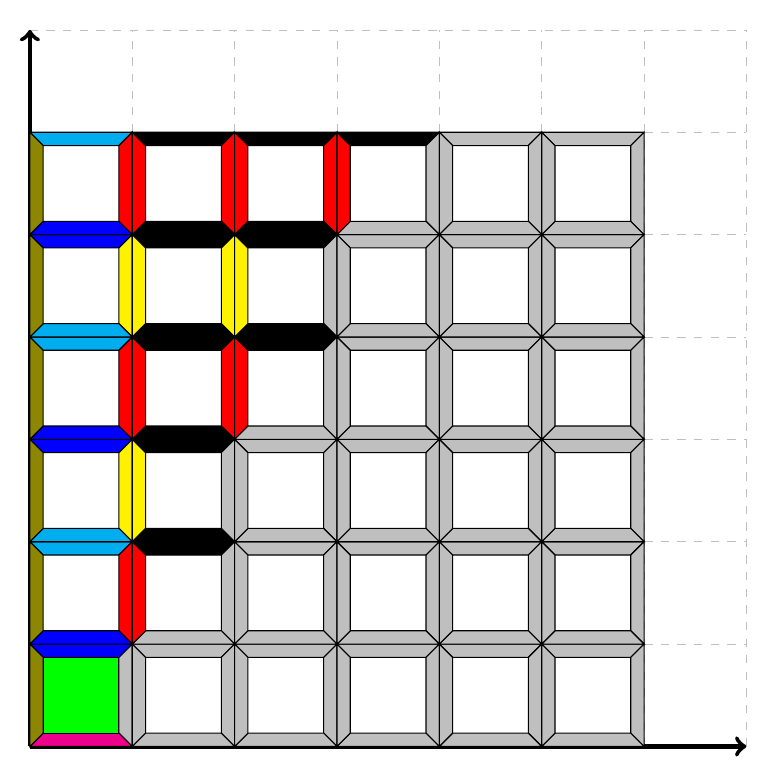
\begin{tikzpicture}[scale=1.3]
\draw[help lines, color=gray!50, dashed] (-3,-3) grid (4,4);
\draw[->,ultra thick] (-3,-3)--(4,-3);
\draw[->,ultra thick] (-3,-3)--(-3,4);
\tikzmath{
  \a = -3;
  \b = -3;
  \side = 1;
  \inc = .13; %% was .2
  }
\filldraw[fill=blue](\a+\side,\b+\side) --(\a+\side-\inc,\b+\side -\inc) --(\a+\inc, \b+\side-\inc)--(\a, \b+\side) --(\a+\side,\b+\side);
\filldraw[fill=lightgray] (\a+\side,\b) -- (\a+\side-\inc,\b+\inc) -- (\a+\side-\inc,\b+\side -\inc) -- (\a+\side,\b+\side) --(\a+\side,\b) ;  
\filldraw[fill=magenta] (\a,\b) -- (\a+\inc,\b+\inc) -- (\a+\side-\inc,\b+\inc)--(\a+\side,\b) --(\a,\b);
\filldraw[fill=olive] (\a,\b+\side)--(\a+\inc,\b-\inc+\side)--(\a+\inc,\b+\inc)--(\a,\b)--(\a,\b+\side);
\filldraw[fill=green] (\a+\inc,\b+\inc) -- (\a+\side-\inc, \b+\inc) -- (\a+\side-\inc,\b+\side-\inc) -- (\a+\inc,\b+\side-\inc) --  (\a+\inc,\b+\inc);
\tikzmath{
  \a = -3;
  \b = -2;
 } 
\filldraw[fill=cyan](\a+\side,\b+\side) --(\a+\side-\inc,\b+\side -\inc) --(\a+\inc, \b+\side-\inc)--(\a, \b+\side) --(\a+\side,\b+\side);
\filldraw[fill=red] (\a+\side,\b) -- (\a+\side-\inc,\b+\inc) -- (\a+\side-\inc,\b+\side -\inc) -- (\a+\side,\b+\side) --(\a+\side,\b) ;  
\filldraw[fill=blue] (\a,\b) -- (\a+\inc,\b+\inc) -- (\a+\side-\inc,\b+\inc)--(\a+\side,\b) --(\a,\b);
\filldraw[fill=olive] (\a,\b+\side)--(\a+\inc,\b-\inc+\side)--(\a+\inc,\b+\inc)--(\a,\b)--(\a,\b+\side);  
\tikzmath{
  \a = -3;
  \b = -1;
 } 
\filldraw[fill=blue](\a+\side,\b+\side) --(\a+\side-\inc,\b+\side -\inc) --(\a+\inc, \b+\side-\inc)--(\a, \b+\side) --(\a+\side,\b+\side);
\filldraw[fill=yellow] (\a+\side,\b) -- (\a+\side-\inc,\b+\inc) -- (\a+\side-\inc,\b+\side -\inc) -- (\a+\side,\b+\side) --(\a+\side,\b) ;  
\filldraw[fill=cyan] (\a,\b) -- (\a+\inc,\b+\inc) -- (\a+\side-\inc,\b+\inc)--(\a+\side,\b) --(\a,\b);
\filldraw[fill=olive] (\a,\b+\side)--(\a+\inc,\b-\inc+\side)--(\a+\inc,\b+\inc)--(\a,\b)--(\a,\b+\side);  
%%
\tikzmath{
  \a = -3;
  \b = 0;
 } 
\filldraw[fill=cyan](\a+\side,\b+\side) --(\a+\side-\inc,\b+\side -\inc) --(\a+\inc, \b+\side-\inc)--(\a, \b+\side) --(\a+\side,\b+\side);
\filldraw[fill=red] (\a+\side,\b) -- (\a+\side-\inc,\b+\inc) -- (\a+\side-\inc,\b+\side -\inc) -- (\a+\side,\b+\side) --(\a+\side,\b) ;  
\filldraw[fill=blue] (\a,\b) -- (\a+\inc,\b+\inc) -- (\a+\side-\inc,\b+\inc)--(\a+\side,\b) --(\a,\b);
\filldraw[fill=olive] (\a,\b+\side)--(\a+\inc,\b-\inc+\side)--(\a+\inc,\b+\inc)--(\a,\b)--(\a,\b+\side);  
\tikzmath{
  \a = -3;
  \b = 1;
 } 
\filldraw[fill=blue](\a+\side,\b+\side) --(\a+\side-\inc,\b+\side -\inc) --(\a+\inc, \b+\side-\inc)--(\a, \b+\side) --(\a+\side,\b+\side);
\filldraw[fill=yellow] (\a+\side,\b) -- (\a+\side-\inc,\b+\inc) -- (\a+\side-\inc,\b+\side -\inc) -- (\a+\side,\b+\side) --(\a+\side,\b) ;  
\filldraw[fill=cyan] (\a,\b) -- (\a+\inc,\b+\inc) -- (\a+\side-\inc,\b+\inc)--(\a+\side,\b) --(\a,\b);
\filldraw[fill=olive] (\a,\b+\side)--(\a+\inc,\b-\inc+\side)--(\a+\inc,\b+\inc)--(\a,\b)--(\a,\b+\side);  
\tikzmath{
  \a = -3;
  \b = 2;
 } 
\filldraw[fill=cyan](\a+\side,\b+\side) --(\a+\side-\inc,\b+\side -\inc) --(\a+\inc, \b+\side-\inc)--(\a, \b+\side) --(\a+\side,\b+\side);
\filldraw[fill=red] (\a+\side,\b) -- (\a+\side-\inc,\b+\inc) -- (\a+\side-\inc,\b+\side -\inc) -- (\a+\side,\b+\side) --(\a+\side,\b) ;  
\filldraw[fill=blue] (\a,\b) -- (\a+\inc,\b+\inc) -- (\a+\side-\inc,\b+\inc)--(\a+\side,\b) --(\a,\b);
\filldraw[fill=olive] (\a,\b+\side)--(\a+\inc,\b-\inc+\side)--(\a+\inc,\b+\inc)--(\a,\b)--(\a,\b+\side);  
%%
\tikzmath{
  \a = -2;
  \b = -3;
 } 
\filldraw[fill=lightgray](\a+\side,\b+\side) --(\a+\side-\inc,\b+\side -\inc) --(\a+\inc, \b+\side-\inc)--(\a, \b+\side) --(\a+\side,\b+\side);
\filldraw[fill=lightgray] (\a+\side,\b) -- (\a+\side-\inc,\b+\inc) -- (\a+\side-\inc,\b+\side -\inc) -- (\a+\side,\b+\side) --(\a+\side,\b) ;  
\filldraw[fill=lightgray] (\a,\b) -- (\a+\inc,\b+\inc) -- (\a+\side-\inc,\b+\inc)--(\a+\side,\b) --(\a,\b);
\filldraw[fill=lightgray] (\a,\b+\side)--(\a+\inc,\b-\inc+\side)--(\a+\inc,\b+\inc)--(\a,\b)--(\a,\b+\side);  
\tikzmath{
  \a = -1;
  \b = -3;
 } 
\filldraw[fill=lightgray](\a+\side,\b+\side) --(\a+\side-\inc,\b+\side -\inc) --(\a+\inc, \b+\side-\inc)--(\a, \b+\side) --(\a+\side,\b+\side);
\filldraw[fill=lightgray] (\a+\side,\b) -- (\a+\side-\inc,\b+\inc) -- (\a+\side-\inc,\b+\side -\inc) -- (\a+\side,\b+\side) --(\a+\side,\b) ;  
\filldraw[fill=lightgray] (\a,\b) -- (\a+\inc,\b+\inc) -- (\a+\side-\inc,\b+\inc)--(\a+\side,\b) --(\a,\b);
\filldraw[fill=lightgray] (\a,\b+\side)--(\a+\inc,\b-\inc+\side)--(\a+\inc,\b+\inc)--(\a,\b)--(\a,\b+\side);  
%
\tikzmath{
  \a = 0;
  \b = -3;
 } 
\filldraw[fill=lightgray](\a+\side,\b+\side) --(\a+\side-\inc,\b+\side -\inc) --(\a+\inc, \b+\side-\inc)--(\a, \b+\side) --(\a+\side,\b+\side);
\filldraw[fill=lightgray] (\a+\side,\b) -- (\a+\side-\inc,\b+\inc) -- (\a+\side-\inc,\b+\side -\inc) -- (\a+\side,\b+\side) --(\a+\side,\b) ;  
\filldraw[fill=lightgray] (\a,\b) -- (\a+\inc,\b+\inc) -- (\a+\side-\inc,\b+\inc)--(\a+\side,\b) --(\a,\b);
\filldraw[fill=lightgray] (\a,\b+\side)--(\a+\inc,\b-\inc+\side)--(\a+\inc,\b+\inc)--(\a,\b)--(\a,\b+\side);  
\tikzmath{
  \a = 1;
  \b = -3;
 } 
\filldraw[fill=lightgray](\a+\side,\b+\side) --(\a+\side-\inc,\b+\side -\inc) --(\a+\inc, \b+\side-\inc)--(\a, \b+\side) --(\a+\side,\b+\side);
\filldraw[fill=lightgray] (\a+\side,\b) -- (\a+\side-\inc,\b+\inc) -- (\a+\side-\inc,\b+\side -\inc) -- (\a+\side,\b+\side) --(\a+\side,\b) ;  
\filldraw[fill=lightgray] (\a,\b) -- (\a+\inc,\b+\inc) -- (\a+\side-\inc,\b+\inc)--(\a+\side,\b) --(\a,\b);
\filldraw[fill=lightgray] (\a,\b+\side)--(\a+\inc,\b-\inc+\side)--(\a+\inc,\b+\inc)--(\a,\b)--(\a,\b+\side);  
\tikzmath{
  \a = 2;
  \b = -3;
 } 
\filldraw[fill=lightgray](\a+\side,\b+\side) --(\a+\side-\inc,\b+\side -\inc) --(\a+\inc, \b+\side-\inc)--(\a, \b+\side) --(\a+\side,\b+\side);
\filldraw[fill=lightgray] (\a+\side,\b) -- (\a+\side-\inc,\b+\inc) -- (\a+\side-\inc,\b+\side -\inc) -- (\a+\side,\b+\side) --(\a+\side,\b) ;  
\filldraw[fill=lightgray] (\a,\b) -- (\a+\inc,\b+\inc) -- (\a+\side-\inc,\b+\inc)--(\a+\side,\b) --(\a,\b);
\filldraw[fill=lightgray] (\a,\b+\side)--(\a+\inc,\b-\inc+\side)--(\a+\inc,\b+\inc)--(\a,\b)--(\a,\b+\side);  
\tikzmath{
  \a = -2;
  \b = -2;
 } 
\filldraw[fill=black](\a+\side,\b+\side) --(\a+\side-\inc,\b+\side -\inc) --(\a+\inc, \b+\side-\inc)--(\a, \b+\side) --(\a+\side,\b+\side);
\filldraw[fill=lightgray] (\a+\side,\b) -- (\a+\side-\inc,\b+\inc) -- (\a+\side-\inc,\b+\side -\inc) -- (\a+\side,\b+\side) --(\a+\side,\b) ;  
\filldraw[fill=lightgray] (\a,\b) -- (\a+\inc,\b+\inc) -- (\a+\side-\inc,\b+\inc)--(\a+\side,\b) --(\a,\b);
\filldraw[fill=red] (\a,\b+\side)--(\a+\inc,\b-\inc+\side)--(\a+\inc,\b+\inc)--(\a,\b)--(\a,\b+\side);  

\tikzmath{
  \a = -1;
  \b = -2;
 } 
\filldraw[fill=lightgray](\a+\side,\b+\side) --(\a+\side-\inc,\b+\side -\inc) --(\a+\inc, \b+\side-\inc)--(\a, \b+\side) --(\a+\side,\b+\side);
\filldraw[fill=lightgray] (\a+\side,\b) -- (\a+\side-\inc,\b+\inc) -- (\a+\side-\inc,\b+\side -\inc) -- (\a+\side,\b+\side) --(\a+\side,\b) ;  
\filldraw[fill=lightgray] (\a,\b) -- (\a+\inc,\b+\inc) -- (\a+\side-\inc,\b+\inc)--(\a+\side,\b) --(\a,\b);
\filldraw[fill=lightgray] (\a,\b+\side)--(\a+\inc,\b-\inc+\side)--(\a+\inc,\b+\inc)--(\a,\b)--(\a,\b+\side);  
%
\tikzmath{
  \a =0;
  \b = -2;
 } 
\filldraw[fill=lightgray](\a+\side,\b+\side) --(\a+\side-\inc,\b+\side -\inc) --(\a+\inc, \b+\side-\inc)--(\a, \b+\side) --(\a+\side,\b+\side);
\filldraw[fill=lightgray] (\a+\side,\b) -- (\a+\side-\inc,\b+\inc) -- (\a+\side-\inc,\b+\side -\inc) -- (\a+\side,\b+\side) --(\a+\side,\b) ;  
\filldraw[fill=lightgray] (\a,\b) -- (\a+\inc,\b+\inc) -- (\a+\side-\inc,\b+\inc)--(\a+\side,\b) --(\a,\b);
\filldraw[fill=lightgray] (\a,\b+\side)--(\a+\inc,\b-\inc+\side)--(\a+\inc,\b+\inc)--(\a,\b)--(\a,\b+\side);  
\tikzmath{
  \a = 1;
  \b = -2;
 } 
\filldraw[fill=lightgray](\a+\side,\b+\side) --(\a+\side-\inc,\b+\side -\inc) --(\a+\inc, \b+\side-\inc)--(\a, \b+\side) --(\a+\side,\b+\side);
\filldraw[fill=lightgray] (\a+\side,\b) -- (\a+\side-\inc,\b+\inc) -- (\a+\side-\inc,\b+\side -\inc) -- (\a+\side,\b+\side) --(\a+\side,\b) ;  
\filldraw[fill=lightgray] (\a,\b) -- (\a+\inc,\b+\inc) -- (\a+\side-\inc,\b+\inc)--(\a+\side,\b) --(\a,\b);
\filldraw[fill=lightgray] (\a,\b+\side)--(\a+\inc,\b-\inc+\side)--(\a+\inc,\b+\inc)--(\a,\b)--(\a,\b+\side);  
\tikzmath{
  \a = 2;
  \b = -2;
 } 
\filldraw[fill=lightgray](\a+\side,\b+\side) --(\a+\side-\inc,\b+\side -\inc) --(\a+\inc, \b+\side-\inc)--(\a, \b+\side) --(\a+\side,\b+\side);
\filldraw[fill=lightgray] (\a+\side,\b) -- (\a+\side-\inc,\b+\inc) -- (\a+\side-\inc,\b+\side -\inc) -- (\a+\side,\b+\side) --(\a+\side,\b) ;  
\filldraw[fill=lightgray] (\a,\b) -- (\a+\inc,\b+\inc) -- (\a+\side-\inc,\b+\inc)--(\a+\side,\b) --(\a,\b);
\filldraw[fill=lightgray] (\a,\b+\side)--(\a+\inc,\b-\inc+\side)--(\a+\inc,\b+\inc)--(\a,\b)--(\a,\b+\side);  

\tikzmath{
  \a = -2;
  \b = -1;
 } 
\filldraw[fill=black](\a+\side,\b+\side) --(\a+\side-\inc,\b+\side -\inc) --(\a+\inc, \b+\side-\inc)--(\a, \b+\side) --(\a+\side,\b+\side);
\filldraw[fill=lightgray] (\a+\side,\b) -- (\a+\side-\inc,\b+\inc) -- (\a+\side-\inc,\b+\side -\inc) -- (\a+\side,\b+\side) --(\a+\side,\b) ;  
\filldraw[fill=black] (\a,\b) -- (\a+\inc,\b+\inc) -- (\a+\side-\inc,\b+\inc)--(\a+\side,\b) --(\a,\b);
\filldraw[fill=yellow] (\a,\b+\side)--(\a+\inc,\b-\inc+\side)--(\a+\inc,\b+\inc)--(\a,\b)--(\a,\b+\side);  

%%
\tikzmath{
  \a = -1;
  \b = -1;
 } 
\filldraw[fill=lightgray](\a+\side,\b+\side) --(\a+\side-\inc,\b+\side -\inc) --(\a+\inc, \b+\side-\inc)--(\a, \b+\side) --(\a+\side,\b+\side);
\filldraw[fill=lightgray] (\a+\side,\b) -- (\a+\side-\inc,\b+\inc) -- (\a+\side-\inc,\b+\side -\inc) -- (\a+\side,\b+\side) --(\a+\side,\b) ;  
\filldraw[fill=lightgray] (\a,\b) -- (\a+\inc,\b+\inc) -- (\a+\side-\inc,\b+\inc)--(\a+\side,\b) --(\a,\b);
\filldraw[fill=lightgray] (\a,\b+\side)--(\a+\inc,\b-\inc+\side)--(\a+\inc,\b+\inc)--(\a,\b)--(\a,\b+\side);  

\tikzmath{
  \a =0;
  \b = -1;
 } 
\filldraw[fill=lightgray](\a+\side,\b+\side) --(\a+\side-\inc,\b+\side -\inc) --(\a+\inc, \b+\side-\inc)--(\a, \b+\side) --(\a+\side,\b+\side);
\filldraw[fill=lightgray] (\a+\side,\b) -- (\a+\side-\inc,\b+\inc) -- (\a+\side-\inc,\b+\side -\inc) -- (\a+\side,\b+\side) --(\a+\side,\b) ;  
\filldraw[fill=lightgray] (\a,\b) -- (\a+\inc,\b+\inc) -- (\a+\side-\inc,\b+\inc)--(\a+\side,\b) --(\a,\b);
\filldraw[fill=lightgray] (\a,\b+\side)--(\a+\inc,\b-\inc+\side)--(\a+\inc,\b+\inc)--(\a,\b)--(\a,\b+\side);  
\tikzmath{
  \a = 1;
  \b = -1;
 } 
\filldraw[fill=lightgray](\a+\side,\b+\side) --(\a+\side-\inc,\b+\side -\inc) --(\a+\inc, \b+\side-\inc)--(\a, \b+\side) --(\a+\side,\b+\side);
\filldraw[fill=lightgray] (\a+\side,\b) -- (\a+\side-\inc,\b+\inc) -- (\a+\side-\inc,\b+\side -\inc) -- (\a+\side,\b+\side) --(\a+\side,\b) ;  
\filldraw[fill=lightgray] (\a,\b) -- (\a+\inc,\b+\inc) -- (\a+\side-\inc,\b+\inc)--(\a+\side,\b) --(\a,\b);
\filldraw[fill=lightgray] (\a,\b+\side)--(\a+\inc,\b-\inc+\side)--(\a+\inc,\b+\inc)--(\a,\b)--(\a,\b+\side);  
\tikzmath{
  \a = 2;
  \b = -1;
 } 
\filldraw[fill=lightgray](\a+\side,\b+\side) --(\a+\side-\inc,\b+\side -\inc) --(\a+\inc, \b+\side-\inc)--(\a, \b+\side) --(\a+\side,\b+\side);
\filldraw[fill=lightgray] (\a+\side,\b) -- (\a+\side-\inc,\b+\inc) -- (\a+\side-\inc,\b+\side -\inc) -- (\a+\side,\b+\side) --(\a+\side,\b) ;  
\filldraw[fill=lightgray] (\a,\b) -- (\a+\inc,\b+\inc) -- (\a+\side-\inc,\b+\inc)--(\a+\side,\b) --(\a,\b);
\filldraw[fill=lightgray] (\a,\b+\side)--(\a+\inc,\b-\inc+\side)--(\a+\inc,\b+\inc)--(\a,\b)--(\a,\b+\side);  

\tikzmath{
  \a = -2;
  \b =0;
 } 
\filldraw[fill=black](\a+\side,\b+\side) --(\a+\side-\inc,\b+\side -\inc) --(\a+\inc, \b+\side-\inc)--(\a, \b+\side) --(\a+\side,\b+\side);
\filldraw[fill=red] (\a+\side,\b) -- (\a+\side-\inc,\b+\inc) -- (\a+\side-\inc,\b+\side -\inc) -- (\a+\side,\b+\side) --(\a+\side,\b) ;  
\filldraw[fill=black] (\a,\b) -- (\a+\inc,\b+\inc) -- (\a+\side-\inc,\b+\inc)--(\a+\side,\b) --(\a,\b);
\filldraw[fill=red] (\a,\b+\side)--(\a+\inc,\b-\inc+\side)--(\a+\inc,\b+\inc)--(\a,\b)--(\a,\b+\side);  

\tikzmath{
  \a = -1;
  \b =0;
 } 
\filldraw[fill=black](\a+\side,\b+\side) --(\a+\side-\inc,\b+\side -\inc) --(\a+\inc, \b+\side-\inc)--(\a, \b+\side) --(\a+\side,\b+\side);
\filldraw[fill=lightgray] (\a+\side,\b) -- (\a+\side-\inc,\b+\inc) -- (\a+\side-\inc,\b+\side -\inc) -- (\a+\side,\b+\side) --(\a+\side,\b) ;  
\filldraw[fill=lightgray] (\a,\b) -- (\a+\inc,\b+\inc) -- (\a+\side-\inc,\b+\inc)--(\a+\side,\b) --(\a,\b);
\filldraw[fill=red] (\a,\b+\side)--(\a+\inc,\b-\inc+\side)--(\a+\inc,\b+\inc)--(\a,\b)--(\a,\b+\side);  

\tikzmath{
  \a =0;
  \b = 0;
 } 
\filldraw[fill=lightgray](\a+\side,\b+\side) --(\a+\side-\inc,\b+\side -\inc) --(\a+\inc, \b+\side-\inc)--(\a, \b+\side) --(\a+\side,\b+\side);
\filldraw[fill=lightgray] (\a+\side,\b) -- (\a+\side-\inc,\b+\inc) -- (\a+\side-\inc,\b+\side -\inc) -- (\a+\side,\b+\side) --(\a+\side,\b) ;  
\filldraw[fill=lightgray] (\a,\b) -- (\a+\inc,\b+\inc) -- (\a+\side-\inc,\b+\inc)--(\a+\side,\b) --(\a,\b);
\filldraw[fill=lightgray] (\a,\b+\side)--(\a+\inc,\b-\inc+\side)--(\a+\inc,\b+\inc)--(\a,\b)--(\a,\b+\side);  
\tikzmath{
  \a = 1;
  \b = 0;
 } 
\filldraw[fill=lightgray](\a+\side,\b+\side) --(\a+\side-\inc,\b+\side -\inc) --(\a+\inc, \b+\side-\inc)--(\a, \b+\side) --(\a+\side,\b+\side);
\filldraw[fill=lightgray] (\a+\side,\b) -- (\a+\side-\inc,\b+\inc) -- (\a+\side-\inc,\b+\side -\inc) -- (\a+\side,\b+\side) --(\a+\side,\b) ;  
\filldraw[fill=lightgray] (\a,\b) -- (\a+\inc,\b+\inc) -- (\a+\side-\inc,\b+\inc)--(\a+\side,\b) --(\a,\b);
\filldraw[fill=lightgray] (\a,\b+\side)--(\a+\inc,\b-\inc+\side)--(\a+\inc,\b+\inc)--(\a,\b)--(\a,\b+\side);  
\tikzmath{
  \a =2;
  \b = 0;
 } 
\filldraw[fill=lightgray](\a+\side,\b+\side) --(\a+\side-\inc,\b+\side -\inc) --(\a+\inc, \b+\side-\inc)--(\a, \b+\side) --(\a+\side,\b+\side);
\filldraw[fill=lightgray] (\a+\side,\b) -- (\a+\side-\inc,\b+\inc) -- (\a+\side-\inc,\b+\side -\inc) -- (\a+\side,\b+\side) --(\a+\side,\b) ;  
\filldraw[fill=lightgray] (\a,\b) -- (\a+\inc,\b+\inc) -- (\a+\side-\inc,\b+\inc)--(\a+\side,\b) --(\a,\b);
\filldraw[fill=lightgray] (\a,\b+\side)--(\a+\inc,\b-\inc+\side)--(\a+\inc,\b+\inc)--(\a,\b)--(\a,\b+\side);  

\tikzmath{
  \a = -2;
  \b =1;
 } 
\filldraw[fill=black](\a+\side,\b+\side) --(\a+\side-\inc,\b+\side -\inc) --(\a+\inc, \b+\side-\inc)--(\a, \b+\side) --(\a+\side,\b+\side);
\filldraw[fill=yellow] (\a+\side,\b) -- (\a+\side-\inc,\b+\inc) -- (\a+\side-\inc,\b+\side -\inc) -- (\a+\side,\b+\side) --(\a+\side,\b) ;  
\filldraw[fill=black] (\a,\b) -- (\a+\inc,\b+\inc) -- (\a+\side-\inc,\b+\inc)--(\a+\side,\b) --(\a,\b);
\filldraw[fill=yellow] (\a,\b+\side)--(\a+\inc,\b-\inc+\side)--(\a+\inc,\b+\inc)--(\a,\b)--(\a,\b+\side);  

\tikzmath{
  \a = -1;
  \b =1;
 } 
\filldraw[fill=black](\a+\side,\b+\side) --(\a+\side-\inc,\b+\side -\inc) --(\a+\inc, \b+\side-\inc)--(\a, \b+\side) --(\a+\side,\b+\side);
\filldraw[fill=lightgray] (\a+\side,\b) -- (\a+\side-\inc,\b+\inc) -- (\a+\side-\inc,\b+\side -\inc) -- (\a+\side,\b+\side) --(\a+\side,\b) ;  
\filldraw[fill=black] (\a,\b) -- (\a+\inc,\b+\inc) -- (\a+\side-\inc,\b+\inc)--(\a+\side,\b) --(\a,\b);
\filldraw[fill=yellow] (\a,\b+\side)--(\a+\inc,\b-\inc+\side)--(\a+\inc,\b+\inc)--(\a,\b)--(\a,\b+\side);  
\tikzmath{
  \a =0;
  \b = 1;
 } 
\filldraw[fill=lightgray](\a+\side,\b+\side) --(\a+\side-\inc,\b+\side -\inc) --(\a+\inc, \b+\side-\inc)--(\a, \b+\side) --(\a+\side,\b+\side);
\filldraw[fill=lightgray] (\a+\side,\b) -- (\a+\side-\inc,\b+\inc) -- (\a+\side-\inc,\b+\side -\inc) -- (\a+\side,\b+\side) --(\a+\side,\b) ;  
\filldraw[fill=lightgray] (\a,\b) -- (\a+\inc,\b+\inc) -- (\a+\side-\inc,\b+\inc)--(\a+\side,\b) --(\a,\b);
\filldraw[fill=lightgray] (\a,\b+\side)--(\a+\inc,\b-\inc+\side)--(\a+\inc,\b+\inc)--(\a,\b)--(\a,\b+\side);  
\tikzmath{
  \a = 1;
  \b = 1;
 } 
\filldraw[fill=lightgray](\a+\side,\b+\side) --(\a+\side-\inc,\b+\side -\inc) --(\a+\inc, \b+\side-\inc)--(\a, \b+\side) --(\a+\side,\b+\side);
\filldraw[fill=lightgray] (\a+\side,\b) -- (\a+\side-\inc,\b+\inc) -- (\a+\side-\inc,\b+\side -\inc) -- (\a+\side,\b+\side) --(\a+\side,\b) ;  
\filldraw[fill=lightgray] (\a,\b) -- (\a+\inc,\b+\inc) -- (\a+\side-\inc,\b+\inc)--(\a+\side,\b) --(\a,\b);
\filldraw[fill=lightgray] (\a,\b+\side)--(\a+\inc,\b-\inc+\side)--(\a+\inc,\b+\inc)--(\a,\b)--(\a,\b+\side);  
\tikzmath{
  \a =2;
  \b = 1;
 } 
\filldraw[fill=lightgray](\a+\side,\b+\side) --(\a+\side-\inc,\b+\side -\inc) --(\a+\inc, \b+\side-\inc)--(\a, \b+\side) --(\a+\side,\b+\side);
\filldraw[fill=lightgray] (\a+\side,\b) -- (\a+\side-\inc,\b+\inc) -- (\a+\side-\inc,\b+\side -\inc) -- (\a+\side,\b+\side) --(\a+\side,\b) ;  
\filldraw[fill=lightgray] (\a,\b) -- (\a+\inc,\b+\inc) -- (\a+\side-\inc,\b+\inc)--(\a+\side,\b) --(\a,\b);
\filldraw[fill=lightgray] (\a,\b+\side)--(\a+\inc,\b-\inc+\side)--(\a+\inc,\b+\inc)--(\a,\b)--(\a,\b+\side);  
\tikzmath{
  \a =-2;
  \b = 2;
 } 
\filldraw[fill=black](\a+\side,\b+\side) --(\a+\side-\inc,\b+\side -\inc) --(\a+\inc, \b+\side-\inc)--(\a, \b+\side) --(\a+\side,\b+\side);
\filldraw[fill=red] (\a+\side,\b) -- (\a+\side-\inc,\b+\inc) -- (\a+\side-\inc,\b+\side -\inc) -- (\a+\side,\b+\side) --(\a+\side,\b) ;  
\filldraw[fill=black] (\a,\b) -- (\a+\inc,\b+\inc) -- (\a+\side-\inc,\b+\inc)--(\a+\side,\b) --(\a,\b);
\filldraw[fill=red] (\a,\b+\side)--(\a+\inc,\b-\inc+\side)--(\a+\inc,\b+\inc)--(\a,\b)--(\a,\b+\side);  
\tikzmath{
  \a =-1;
  \b = 2;
 } 
\filldraw[fill=black](\a+\side,\b+\side) --(\a+\side-\inc,\b+\side -\inc) --(\a+\inc, \b+\side-\inc)--(\a, \b+\side) --(\a+\side,\b+\side);
\filldraw[fill=red] (\a+\side,\b) -- (\a+\side-\inc,\b+\inc) -- (\a+\side-\inc,\b+\side -\inc) -- (\a+\side,\b+\side) --(\a+\side,\b) ;  
\filldraw[fill=black] (\a,\b) -- (\a+\inc,\b+\inc) -- (\a+\side-\inc,\b+\inc)--(\a+\side,\b) --(\a,\b);
\filldraw[fill=red] (\a,\b+\side)--(\a+\inc,\b-\inc+\side)--(\a+\inc,\b+\inc)--(\a,\b)--(\a,\b+\side);  
\tikzmath{
  \a =0;
  \b = 2;
 } 
\filldraw[fill=black](\a+\side,\b+\side) --(\a+\side-\inc,\b+\side -\inc) --(\a+\inc, \b+\side-\inc)--(\a, \b+\side) --(\a+\side,\b+\side);
\filldraw[fill=lightgray] (\a+\side,\b) -- (\a+\side-\inc,\b+\inc) -- (\a+\side-\inc,\b+\side -\inc) -- (\a+\side,\b+\side) --(\a+\side,\b) ;  
\filldraw[fill=lightgray] (\a,\b) -- (\a+\inc,\b+\inc) -- (\a+\side-\inc,\b+\inc)--(\a+\side,\b) --(\a,\b);
\filldraw[fill=red] (\a,\b+\side)--(\a+\inc,\b-\inc+\side)--(\a+\inc,\b+\inc)--(\a,\b)--(\a,\b+\side);  
\tikzmath{
  \a = 1;
  \b = 2;
 } 
\filldraw[fill=lightgray](\a+\side,\b+\side) --(\a+\side-\inc,\b+\side -\inc) --(\a+\inc, \b+\side-\inc)--(\a, \b+\side) --(\a+\side,\b+\side);
\filldraw[fill=lightgray] (\a+\side,\b) -- (\a+\side-\inc,\b+\inc) -- (\a+\side-\inc,\b+\side -\inc) -- (\a+\side,\b+\side) --(\a+\side,\b) ;  
\filldraw[fill=lightgray] (\a,\b) -- (\a+\inc,\b+\inc) -- (\a+\side-\inc,\b+\inc)--(\a+\side,\b) --(\a,\b);
\filldraw[fill=lightgray] (\a,\b+\side)--(\a+\inc,\b-\inc+\side)--(\a+\inc,\b+\inc)--(\a,\b)--(\a,\b+\side);  
\tikzmath{
  \a =2;
  \b = 2;
 } 
\filldraw[fill=lightgray](\a+\side,\b+\side) --(\a+\side-\inc,\b+\side -\inc) --(\a+\inc, \b+\side-\inc)--(\a, \b+\side) --(\a+\side,\b+\side);
\filldraw[fill=lightgray] (\a+\side,\b) -- (\a+\side-\inc,\b+\inc) -- (\a+\side-\inc,\b+\side -\inc) -- (\a+\side,\b+\side) --(\a+\side,\b) ;  
\filldraw[fill=lightgray] (\a,\b) -- (\a+\inc,\b+\inc) -- (\a+\side-\inc,\b+\inc)--(\a+\side,\b) --(\a,\b);
\filldraw[fill=lightgray] (\a,\b+\side)--(\a+\inc,\b-\inc+\side)--(\a+\inc,\b+\inc)--(\a,\b)--(\a,\b+\side);  

\end{tikzpicture}
\end{array}$
\end{flushleft}






\vfil\eject


\begin{flushleft}  
$\begin{array}{lllll}
\tikzmath{
  \a = -3;
  \b = -3;
  }
\begin{tikzpicture}[scale=1.3]  
\filldraw[fill=blue](\a+\side,\b+\side) --(\a+\side-\inc,\b+\side -\inc) --(\a+\inc, \b+\side-\inc)--(\a, \b+\side) --(\a+\side,\b+\side);
\filldraw[fill=lightgray] (\a+\side,\b) -- (\a+\side-\inc,\b+\inc) -- (\a+\side-\inc,\b+\side -\inc) -- (\a+\side,\b+\side) --(\a+\side,\b) ;  
\filldraw[fill=magenta] (\a,\b) -- (\a+\inc,\b+\inc) -- (\a+\side-\inc,\b+\inc)--(\a+\side,\b) --(\a,\b);
\filldraw[fill=olive] (\a,\b+\side)--(\a+\inc,\b-\inc+\side)--(\a+\inc,\b+\inc)--(\a,\b)--(\a,\b+\side);
\filldraw[fill=green] (\a+\inc,\b+\inc) -- (\a+\side-\inc, \b+\inc) -- (\a+\side-\inc,\b+\side-\inc) -- (\a+\inc,\b+\side-\inc) --  (\a+\inc,\b+\inc);
\tikzmath{
  \a = -1.5;
  \b = -3;
 } 
\filldraw[fill=lightgray](\a+\side,\b+\side) --(\a+\side-\inc,\b+\side -\inc) --(\a+\inc, \b+\side-\inc)--(\a, \b+\side) --(\a+\side,\b+\side);
\filldraw[fill=lightgray] (\a+\side,\b) -- (\a+\side-\inc,\b+\inc) -- (\a+\side-\inc,\b+\side -\inc) -- (\a+\side,\b+\side) --(\a+\side,\b) ;  
\filldraw[fill=lightgray] (\a,\b) -- (\a+\inc,\b+\inc) -- (\a+\side-\inc,\b+\inc)--(\a+\side,\b) --(\a,\b);
\filldraw[fill=lightgray] (\a,\b+\side)--(\a+\inc,\b-\inc+\side)--(\a+\inc,\b+\inc)--(\a,\b)--(\a,\b+\side);  
\tikzmath{
  \a = 0;
  \b = -3;
 } 
\filldraw[fill=cyan](\a+\side,\b+\side) --(\a+\side-\inc,\b+\side -\inc) --(\a+\inc, \b+\side-\inc)--(\a, \b+\side) --(\a+\side,\b+\side);
\filldraw[fill=red] (\a+\side,\b) -- (\a+\side-\inc,\b+\inc) -- (\a+\side-\inc,\b+\side -\inc) -- (\a+\side,\b+\side) --(\a+\side,\b) ;  
\filldraw[fill=blue] (\a,\b) -- (\a+\inc,\b+\inc) -- (\a+\side-\inc,\b+\inc)--(\a+\side,\b) --(\a,\b);
\filldraw[fill=olive] (\a,\b+\side)--(\a+\inc,\b-\inc+\side)--(\a+\inc,\b+\inc)--(\a,\b)--(\a,\b+\side);  
\tikzmath{
  \a = -3;
  \b =-1.5;
 } 
\filldraw[fill=black](\a+\side,\b+\side) --(\a+\side-\inc,\b+\side -\inc) --(\a+\inc, \b+\side-\inc)--(\a, \b+\side) --(\a+\side,\b+\side);
\filldraw[fill=red] (\a+\side,\b) -- (\a+\side-\inc,\b+\inc) -- (\a+\side-\inc,\b+\side -\inc) -- (\a+\side,\b+\side) --(\a+\side,\b) ;  
\filldraw[fill=black] (\a,\b) -- (\a+\inc,\b+\inc) -- (\a+\side-\inc,\b+\inc)--(\a+\side,\b) --(\a,\b);
\filldraw[fill=red] (\a,\b+\side)--(\a+\inc,\b-\inc+\side)--(\a+\inc,\b+\inc)--(\a,\b)--(\a,\b+\side);  
\tikzmath{
  \a = -1.5;
  \b = -1.5;
 } 
\filldraw[fill=blue](\a+\side,\b+\side) --(\a+\side-\inc,\b+\side -\inc) --(\a+\inc, \b+\side-\inc)--(\a, \b+\side) --(\a+\side,\b+\side);
\filldraw[fill=yellow] (\a+\side,\b) -- (\a+\side-\inc,\b+\inc) -- (\a+\side-\inc,\b+\side -\inc) -- (\a+\side,\b+\side) --(\a+\side,\b) ;  
\filldraw[fill=cyan] (\a,\b) -- (\a+\inc,\b+\inc) -- (\a+\side-\inc,\b+\inc)--(\a+\side,\b) --(\a,\b);
\filldraw[fill=olive] (\a,\b+\side)--(\a+\inc,\b-\inc+\side)--(\a+\inc,\b+\inc)--(\a,\b)--(\a,\b+\side);  
\tikzmath{
  \a = 0;
  \b =-1.5;
 } 
\filldraw[fill=black](\a+\side,\b+\side) --(\a+\side-\inc,\b+\side -\inc) --(\a+\inc, \b+\side-\inc)--(\a, \b+\side) --(\a+\side,\b+\side);
\filldraw[fill=yellow] (\a+\side,\b) -- (\a+\side-\inc,\b+\inc) -- (\a+\side-\inc,\b+\side -\inc) -- (\a+\side,\b+\side) --(\a+\side,\b) ;  
\filldraw[fill=black] (\a,\b) -- (\a+\inc,\b+\inc) -- (\a+\side-\inc,\b+\inc)--(\a+\side,\b) --(\a,\b);
\filldraw[fill=yellow] (\a,\b+\side)--(\a+\inc,\b-\inc+\side)--(\a+\inc,\b+\inc)--(\a,\b)--(\a,\b+\side);  
\tikzmath{
  \a = 1.5;
  \b =-3;
 } 
\filldraw[fill=black](\a+\side,\b+\side) --(\a+\side-\inc,\b+\side -\inc) --(\a+\inc, \b+\side-\inc)--(\a, \b+\side) --(\a+\side,\b+\side);
\filldraw[fill=lightgray] (\a+\side,\b) -- (\a+\side-\inc,\b+\inc) -- (\a+\side-\inc,\b+\side -\inc) -- (\a+\side,\b+\side) --(\a+\side,\b) ;  
\filldraw[fill=lightgray] (\a,\b) -- (\a+\inc,\b+\inc) -- (\a+\side-\inc,\b+\inc)--(\a+\side,\b) --(\a,\b);
\filldraw[fill=red] (\a,\b+\side)--(\a+\inc,\b-\inc+\side)--(\a+\inc,\b+\inc)--(\a,\b)--(\a,\b+\side);  
\tikzmath{
  \a = 1.5;
  \b =-1.5;
 } 
\filldraw[fill=black](\a+\side,\b+\side) --(\a+\side-\inc,\b+\side -\inc) --(\a+\inc, \b+\side-\inc)--(\a, \b+\side) --(\a+\side,\b+\side);
\filldraw[fill=lightgray] (\a+\side,\b) -- (\a+\side-\inc,\b+\inc) -- (\a+\side-\inc,\b+\side -\inc) -- (\a+\side,\b+\side) --(\a+\side,\b) ;  
\filldraw[fill=black] (\a,\b) -- (\a+\inc,\b+\inc) -- (\a+\side-\inc,\b+\inc)--(\a+\side,\b) --(\a,\b);
\filldraw[fill=yellow] (\a,\b+\side)--(\a+\inc,\b-\inc+\side)--(\a+\inc,\b+\inc)--(\a,\b)--(\a,\b+\side);  



\end{tikzpicture}
\end{array}
$
\end{flushleft}

\vfil\eject




 \begin{flushleft}
$\begin{array}{l}
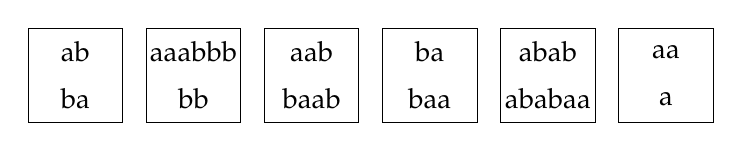
\begin{tikzpicture}[scale=.6]
\foreach \x in {0,2.5,5,7.5,10,12.5}
\foreach \y in {0}
{
\draw (\x, \y)    rectangle ++(2,2);
};
\draw  (11,1.5) node{abab};  %% north
\draw  (11,.5) node{ababaa};  %% south
%
\draw  (3.5,1.5) node{aaabbb};  %% north
\draw  (3.5,.5) node{bb};  %% south
 %
 \draw  (6,1.5) node{aab};  %% north
\draw  (6,.5) node{baab};  %% south
%
\draw  (8.5,1.5) node{ba};  %% north
\draw  (8.5,.5) node{baa};  %% south
% \draw  (6,1.7) node{$\one$};  %% north
%draw (6.7,1) node{$\addone$}; %% east
%\draw  (6,.3) node{$\one$};  %% south
 %\draw  (5.3,1) node{$\addone$};   %% west
 %
%\draw  (8.5,1.7) node{$\one$};  %% north
%\draw (9.2,1) node{$\addhash$}; %% east
%\draw  (8.5,.3) node{$\one$};  %% south
 %\draw  (7.8,1) node{$\addhash$};   %% west
 %
\draw  (1,1.5) node{ab};  %% north
\draw (1,.5) node{ba}; %% east
%
\draw  (13.5,1.5) node{aa};  %% north
\draw  (13.5,.5) node{a};  %% south
 \end{tikzpicture}
\end{array}$ 
\end{flushleft}


 \begin{flushleft}
$\begin{array}{l}
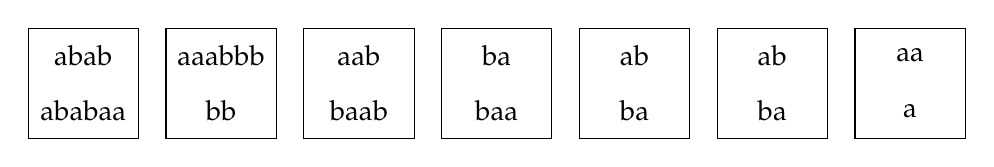
\begin{tikzpicture}[scale=.7]
\foreach \x in {0,2.5,5,7.5,10,12.5,15}
\foreach \y in {0}
{
\draw (\x, \y)    rectangle ++(2,2);
};
%%%
%
\draw  (3.5,1.5) node{aaabbb};  %% north
\draw  (3.5,.5) node{bb};  %% south
 %
 \draw  (6,1.5) node{aab};  %% north
\draw  (6,.5) node{baab};  %% south
%
\draw  (8.5,1.5) node{ba};  %% north
\draw  (8.5,.5) node{baa};  %% south
% \draw  (6,1.7) node{$\one$};  %% north
%draw (6.7,1) node{$\addone$}; %% east
%\draw  (6,.3) node{$\one$};  %% south
 %\draw  (5.3,1) node{$\addone$};   %% west
 %
%\draw  (8.5,1.7) node{$\one$};  %% north
%\draw (9.2,1) node{$\addhash$}; %% east
%\draw  (8.5,.3) node{$\one$};  %% south
 %\draw  (7.8,1) node{$\addhash$};   %% west
 %
 \draw  (1,1.5) node{abab};  %% north
\draw  (1,.5) node{ababaa};  %% south

 \draw  (11,1.5) node{ab};  %% north
\draw (11,.5) node{ba}; %% east

\draw  (13.5,1.5) node{ab};  %% north
\draw  (13.5,.5) node{ba};  %% south

\draw  (16,1.5) node{aa};  %% north
\draw  (16,.5) node{a};  %% south

 \end{tikzpicture}
 \end{array}$ 
\end{flushleft}



 \begin{flushleft}
$\begin{array}{l}
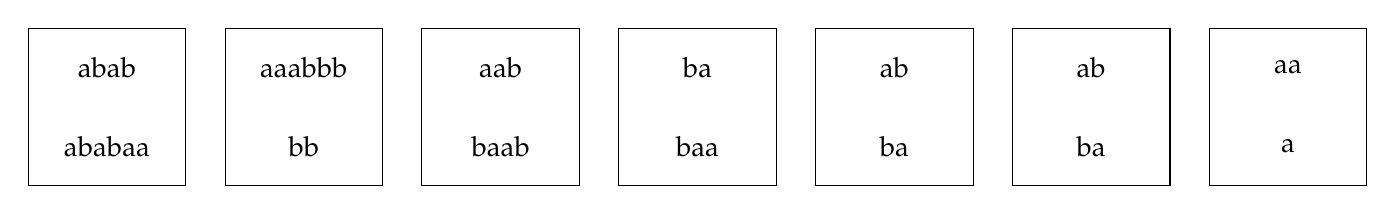
\begin{tikzpicture}
\foreach \x in {0,2.5,5,7.5,10,12.5,15}
\foreach \y in {0}
{
\draw (\x, \y)    rectangle ++(2,2);
};
%%%
%
\draw  (3.5,1.5) node{aaabbb};  %% north
\draw  (3.5,.5) node{bb};  %% south
 %
 \draw  (6,1.5) node{aab};  %% north
\draw  (6,.5) node{baab};  %% south
%
\draw  (8.5,1.5) node{ba};  %% north
\draw  (8.5,.5) node{baa};  %% south
% \draw  (6,1.7) node{$\one$};  %% north
%draw (6.7,1) node{$\addone$}; %% east
%\draw  (6,.3) node{$\one$};  %% south
 %\draw  (5.3,1) node{$\addone$};   %% west
 %
%\draw  (8.5,1.7) node{$\one$};  %% north
%\draw (9.2,1) node{$\addhash$}; %% east
%\draw  (8.5,.3) node{$\one$};  %% south
 %\draw  (7.8,1) node{$\addhash$};   %% west
 %
 \draw  (1,1.5) node{abab};  %% north
\draw  (1,.5) node{ababaa};  %% south

 \draw  (11,1.5) node{ab};  %% north
\draw (11,.5) node{ba}; %% east

\draw  (13.5,1.5) node{ab};  %% north
\draw  (13.5,.5) node{ba};  %% south

\draw  (16,1.5) node{aa};  %% north
\draw  (16,.5) node{a};  %% south

 \end{tikzpicture}
\end{array}$ 
\end{flushleft}

\vfil\eject

 \begin{flushleft}
$\begin{array}{l}
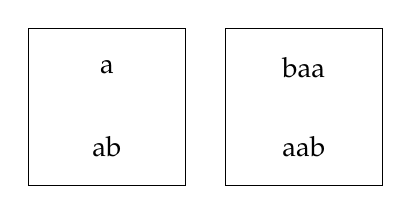
\begin{tikzpicture}
\foreach \x in {0,2.5}
\foreach \y in {0}
{
\draw (\x, \y)    rectangle ++(2,2);
};
%%%
%
 \draw  (1,1.5) node{a};  %% north
\draw  (1,.5) node{ab};  %% south
\draw  (3.5,1.5) node{baa};  %% north
\draw  (3.5,.5) node{aab};  %% south
\end{tikzpicture}
 \end{array}
$
\end{flushleft}
then $f(I)$ would be the $PCP$ instance
  \begin{flushleft}
  $
\begin{array}{l}
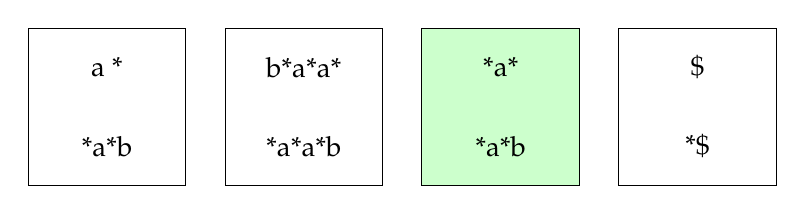
\begin{tikzpicture}
 \filldraw[fill=green!20,draw=green!50!black] (5,0)    rectangle ++(2,2);
\foreach \x in {0,2.5,5,7.5}
\foreach \y in {0}
{
\draw (\x, \y)    rectangle ++(2,2);
};
%%%
%
 \draw  (1,1.5) node{a *};  %% north
\draw  (1,.5) node{*a*b};  %% south
\draw  (3.5,1.5) node{b*a*a*};  %% north
\draw  (3.5,.5) node{*a*a*b};  %% south
 \draw  (6,1.5) node{*a*};  %% north
\draw  (6,.5) node{*a*b};  %% south
\draw  (8.5,1.5) node{\$};  %% north
\draw  (8.5,.5) node{*\$};  %% southf
\end{tikzpicture}
\end{array}$ 
 \end{flushleft}

\vfil\eject
\begin{flushleft}
$
\begin{array}{l}
 \dominogreen{start}{start\ \numberone}
\quad
\dominothin{\one}{\one}
\quad
\dominothin{\hash}{\hash}
\end{array}
$
\end{flushleft}

\vfil\eject
\begin{flushleft}
$
\begin{array}{ll}
 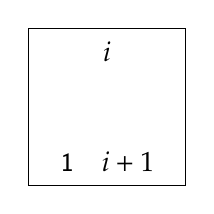
\begin{tikzpicture}
\foreach \x in {0}
\foreach \y in {0}
{
\draw (\x, \y)    rectangle ++(2,2);
};
\draw  (1,1.7) node{$i$};  %% north
%\draw (1.7,1) node{$\passthrough$}; %% east
\draw  (1,.3) node{\one\quad  $i+1$};  %% south
 %\draw  (.3,1) node{$\passthrough$};   %% west
 %
\end{tikzpicture}
&\qquad\qquad\qquad
 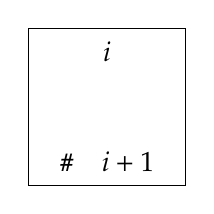
\begin{tikzpicture}
\foreach \x in {0}
\foreach \y in {0}
{
\draw (\x, \y)    rectangle ++(2,2);
};
\draw  (1,1.7) node{$i$};  %% north
%\draw (1.7,1) node{$\passthrough$}; %% east
\draw  (1,.3) node{\hash\quad $i+1$};  %% south
 %\draw  (.3,1) node{$\passthrough$};   %% west
 %
\end{tikzpicture}
\end{array}
$
\end{flushleft}

\vfil\eject





\vfil\eject

\begin{flushleft}
$
\begin{array}{ll}
 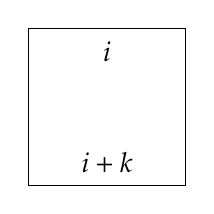
\begin{tikzpicture}
\foreach \x in {0}
\foreach \y in {0}
{
\draw (\x, \y)    rectangle ++(2,2);
};
\draw  (1,1.7) node{$i$};  %% north
%\draw (1.7,1) node{$\passthrough$}; %% east
\draw  (1,.3) node{$i+k$};  %% south
 %\draw  (.3,1) node{$\passthrough$};   %% west
 %
\end{tikzpicture}
&\qquad\qquad\qquad
 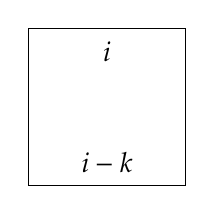
\begin{tikzpicture}
\foreach \x in {0}
\foreach \y in {0}
{
\draw (\x, \y)    rectangle ++(2,2);
};
\draw  (1,1.7) node{$i$};  %% north
%\draw (1.7,1) node{$\passthrough$}; %% east
\draw  (1,.3) node{$i-k$};  %% south
 %\draw  (.3,1) node{$\passthrough$};   %% west
 %
\end{tikzpicture}
\end{array}
$
\end{flushleft}

\vfil\eject


\begin{flushleft}
$\domino{i}{i+1}%quad\mbox{halt}}{\mbox{halt}}
 \quad
 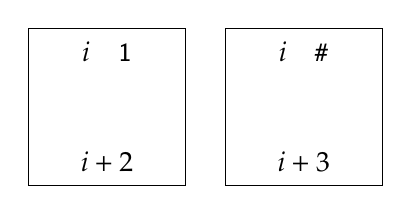
\begin{tikzpicture}
\foreach \x in {0,2.5}
\foreach \y in {0}
{
\draw (\x, \y)    rectangle ++(2,2);
};
\draw  (1,1.7) node{$i\quad {\one}$};  %% north
%\draw (1.7,1) node{$\addone$}; %% east
\draw  (1,.3) node{$i+2$};  %% south
 %\draw  (.3,1) node{$\addone$};   %% west
 %
\draw  (3.5,1.7) node{$i\quad  {\hash}$};  %% north
%\draw (4.2,1) node{$\addone$}; %% east
\draw  (3.5,.3) node{$i+3$};  %% south
% \draw  (2.8,1) node{$\one$};   %% west
 %
  \end{tikzpicture}
$
\end{flushleft}

\vfil\eject


\begin{flushleft}
$
\begin{array}{l}
\dominogreen{start}{start\ \numberone}
\quad
\dominothin{\one}{\one}
\quad
\dominothin{\hash}{\hash}
\quad
\domino{2\, \  halt}{halt}
\quad
 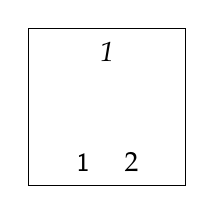
\begin{tikzpicture}
\foreach \x in {0}
\foreach \y in {0}
{
\draw (\x, \y)    rectangle ++(2,2);
};
\draw  (1,1.7) node{$\numberone$};  %% north
%\draw (1.7,1) node{$\passthrough$}; %% east
\draw  (1,.3) node{$\one$ \quad $2$};  %% south
 %\draw  (.3,1) node{$\passthrough$};   %% west
 %
\end{tikzpicture}
\end{array}
$
\end{flushleft}

\vfil\eject




\begin{flushleft}
$\begin{array}{l}
\dominogreen{start}{start\ \numberone}
\quad
\dominothin{\one}{\one}
\quad
\dominothin{\hash}{\hash}
\quad
\domino{3\, \  halt}{halt}
\quad
 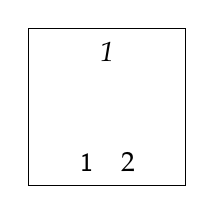
\begin{tikzpicture}
\foreach \x in {0}
\foreach \y in {0}
{
\draw (\x, \y)    rectangle ++(2,2);
};
\draw  (1,1.7) node{$\numberone$};  %% north
%\draw (1.7,1) node{$\passthrough$}; %% east
\draw  (1,.3) node{$\one$\quad $2$};  %% south
 %\draw  (.3,1) node{$\passthrough$};   %% west
 %
\end{tikzpicture}
\quad
 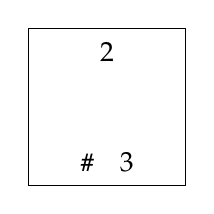
\begin{tikzpicture}
\foreach \x in {0}
\foreach \y in {0}
{
\draw (\x, \y)    rectangle ++(2,2);
};
\draw  (1,1.7) node{$2$};  %% north
%\draw (1.7,1) node{$\passthrough$}; %% east
\draw  (1,.3) node{$\hash$ \ \, $3$};  %% south
 %\draw  (.3,1) node{$\passthrough$};   %% west
 %
\end{tikzpicture}
\end{array}
$
\end{flushleft}

\vfil\eject



\begin{flushleft}
$\begin{array}{l}
\one\hash\hash | \one \hash^5  | \one^3\hash^3 |  \one^2 \hash^4  |  \one^3 \hash^4
\end{array}$
\end{flushleft}

asdf


\begin{flushleft}
$
\begin{array}{l}
\dominogreen{start}{start\ \numberone}
\quad
\dominothin{\one}{\one}
\quad
\dominothin{\hash}{\hash}
\quad
\domino{7\, \  halt}{halt}
\\
 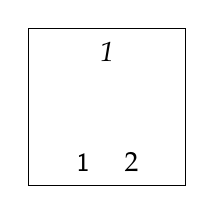
\begin{tikzpicture}
\foreach \x in {0}
\foreach \y in {0}
{
\draw (\x, \y)    rectangle ++(2,2);
};
\draw  (1,1.7) node{$\numberone$};  %% north
%\draw (1.7,1) node{$\passthrough$}; %% east
\draw  (1,.3) node{$\one$ \quad $2$};  %% south
 %\draw  (.3,1) node{$\passthrough$};   %% west
 %
\end{tikzpicture}
\quad
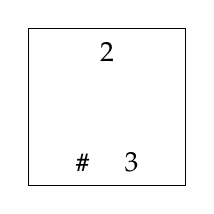
\begin{tikzpicture}
\foreach \x in {0}
\foreach \y in {0}
{
\draw (\x, \y)    rectangle ++(2,2);
};
\draw  (1,1.7) node{$2$};  %% north
%\draw (1.7,1) node{$\passthrough$}; %% east
\draw  (1,.3) node{$\hash$ \quad $3$};  %% south
 %\draw  (.3,1) node{$\passthrough$};   %% west
 %
\end{tikzpicture}
\\
\domino{3}{4}
\quad 
\domino{3\, \quad  \one}{5}
\quad 
\domino{3\, \quad  \hash}{6}
\\
\domino{4}{7} 
\quad
\domino{5}{3} 
\quad
\domino{6}{3} 
\quad
\end{array}
$
\end{flushleft}

\vfil\eject


 



\begin{flushleft}
$\begin{array}{l}

\end{array}
$
\end{flushleft}

\vfil\eject


 

 



\begin{flushleft}
$\begin{array}{l}

\end{array}
$
\end{flushleft}

\vfil\eject


 


 



\begin{flushleft}
$\begin{array}{l}

\end{array}
$
\end{flushleft}

\vfil\eject


 


 



\begin{flushleft}
$\begin{array}{l}

\end{array}
$
\end{flushleft}

\vfil\eject


 


 



\begin{flushleft}
$\begin{array}{l}
\begin{array}{l}
\dominogreen{start}{start\ \numberone}
\quad
\domino{\numberone}{\one\quad 2}
\quad
\dominothin{\one}{\one}
\quad

\domino{2}{\hash\quad 3}
\quad
\dominothin{\one}{\one}
\quad
\dominothin{\hash}{\hash}\\
\domino{3\quad \one}{5}
\quad
\dominothin{\hash}{\hash}
\quad
\dominothin{5}{3}
\quad
\dominothin{\hash}{\hash}
\\
\domino{3\quad \hash}{6}
\quad
\domino{6}{3}
\\
\domino{3}{4}
\quad
\domino{4}{7}
\quad
\domino{7\quad halt}{halt}
\end{array}

\end{array}
$
\end{flushleft}

\vfil\eject


 


 



\begin{flushleft}
$\begin{array}{l}
start\ \numberone \one\  2 \one\hash\ 3 \one \hash \ 5\hash\ 3\hash\ 6\ 3 \ 4\ 7
\end{array}
$
\end{flushleft}

\vfil\eject


 


 



\begin{flushleft}
$\begin{array}{l}
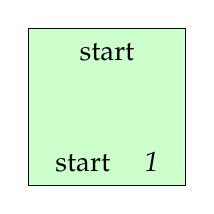
\begin{tikzpicture}
 \filldraw[fill=green!20,draw=green!50!black] (0,0)    rectangle ++(2,2);
\foreach \x in {0}
\foreach \y in {0}
{
\draw (\x, \y)    rectangle ++(2,2);
};
\draw  (1,1.7) node{start};  %% north
%\draw (1.7,1) node{$\addone$}; %% east
\draw  (1,.3) node{start \quad \numberone};  %% south
\end{tikzpicture}
\end{array}
$
\end{flushleft}

\vfil\eject
%And next to it, we only have one choice
\begin{flushleft}
$\begin{array}{l}
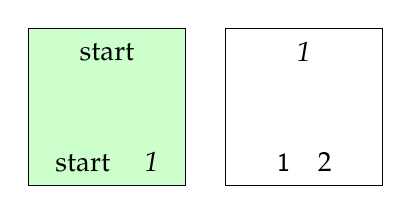
\begin{tikzpicture}
 \filldraw[fill=green!20,draw=green!50!black] (0,0)    rectangle ++(2,2);
\foreach \x in {0,2.5}
\foreach \y in {0}
{
\draw (\x, \y)    rectangle ++(2,2);
};
%\draw (1.7,1) node{$\addone$}; %% east
\draw  (1,1.7) node{start};  %% north
%\draw (1.7,1) node{$\addone$}; %% east
\draw  (1,.3) node{start \quad \numberone};  %% south
\draw  (3.5,1.7) node{$\numberone$};  %% north
%\draw (4.2,1) node{$\addone$}; %% east
\draw  (3.5,.3) node{$\one$\quad 2};  %% south
\end{tikzpicture}
\end{array}
$
\end{flushleft}

\vfil\eject


 


 



\begin{flushleft}
$\begin{array}{l}
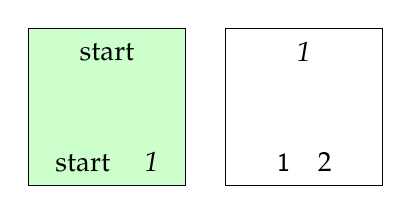
\begin{tikzpicture}
 \filldraw[fill=green!20,draw=green!50!black] (0,0)    rectangle ++(2,2);
\foreach \x in {0,2.5}
\foreach \y in {0}
{
\draw (\x, \y)    rectangle ++(2,2);
};
\draw  (1,1.7) node{start};  %% north
%\draw (1.7,1) node{$\addone$}; %% east
\draw  (1,.3) node{start \quad \numberone};  %% south
\draw  (3.5,1.7) node{$\numberone$};  %% north
%\draw (4.2,1) node{$\addone$}; %% east
\draw  (3.5,.3) node{$\one$\quad 2};  %% south
\end{tikzpicture}

\end{array}
$
\end{flushleft}

\vfil\eject


 


 

\begin{flushleft}
$\begin{array}{l}
\dominogreen{start}{start\quad\numberone}
\
\domino{\numberone}{\one\quad 2}
\
\dominothin{\one}{\one}
\
\domino{2}{\hash\quad 3}
\end{array}
$
\end{flushleft}

\vfil\eject


 


 



\begin{flushleft}
$\begin{array}{l}
\dominogreen{start}{start\quad\numberone}
\
\domino{\numberone}{\one\quad 2}
\
\dominothin{\one}{\one}
\
\domino{2}{\hash\quad 3}
\
\dominothin{\one}{\one}
\
\dominothin{\hash}{\hash}
\end{array}
$
\end{flushleft}

\vfil\eject


 



\begin{flushleft}
$\begin{array}{l}
\dominogreen{start}{start\quad\numberone}
\
\domino{\numberone}{\one\quad 2}
\
\dominothin{\one}{\one}
\
\domino{2}{\hash\quad 3}
\
\dominothin{\one}{\one}
\
\dominothin{\hash}{\hash}
\\
\domino{3}{\hash\quad 4}
\
\dominothin{\one}{\inverse{\one}}
\
\dominothin{\hash}{\hash}
\
\dominothin{\hash}{\hash}
\
\domino{4\quad \inverse{\one}}{3}
\
\dominothin{\hash}{\hash}
\
\dominothin{\hash}{\hash}
\
\\
\domino{3}{\hash\quad 4}
\
\
\dominothin{\hash}{\inverse{\hash}}
\
\dominothin{\hash}{\hash}
\
\dominothin{\hash}{\hash}
\\
\domino{4\quad \inverse{\hash}}{4}
\
\dominothin{\hash}{\inverse{\hash}}
\
\dominothin{\hash}{\hash}
\
\domino{4\quad \inverse{\hash}}{4}
\
\dominothin{\hash}{\inverse{\hash}}
\
\domino{4\quad \inverse{\hash}}{4}
\
\domino{4\quad halt}{halt}
\end{array}
$
\end{flushleft}

\vfil\eject


 


 



\begin{flushleft}
$\begin{array}{l}
\cdots \quad
\domino{?}{k}
\quad
\domino{k}{N+1}
\\ \\
%%%and we get a Post word by adding on the ``halting'' domino:
\cdots \quad
\domino{?}{k}
\quad
\domino{k}{N+1}
\quad
\domino{N+1\ \, halt}{halt}
\end{array}
$
\end{flushleft}

\vfil\eject


 


 



\begin{flushleft}
$\begin{array}{l}
 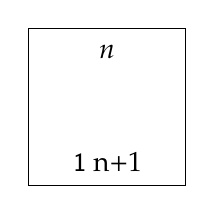
\begin{tikzpicture}
\foreach \x in {0}
\foreach \y in {0}
{
\draw (\x, \y)    rectangle ++(2,2);
};
\draw  (1,1.7) node{$n$};  %% north
%\draw (1.7,1) node{$\passthrough$}; %% east
\draw  (1,.3) node{\one\  n+1};  %% south
 %\draw  (.3,1) node{$\passthrough$};   %% west
 %
\end{tikzpicture}
\end{array}
$
\end{flushleft}

\vfil\eject


 
\begin{flushleft}
$\begin{array}{l}
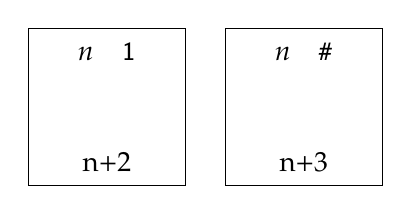
\begin{tikzpicture}
\foreach \x in {0,2.5}
\foreach \y in {0}
{
\draw (\x, \y)    rectangle ++(2,2);
};
\draw  (1,1.7) node{$n\quad  {\one}$};  %% north
%\draw (1.7,1) node{$\addone$}; %% east
\draw  (1,.3) node{n+2};  %% south
 %\draw  (.3,1) node{$\addone$};   %% west
 %
\draw  (3.5,1.7) node{$n\quad  {\hash}$};  %% north
%\draw (4.2,1) node{$\addone$}; %% east
\draw  (3.5,.3) node{n+3};  %% south
% \draw  (2.8,1) node{$\one$};   %% west
 %
  \end{tikzpicture}
\end{array}$
\end{flushleft}

\vfil\eject




\begin{flushleft}
$
\begin{array}{ccccc}
\domino{}{i} 
 \begin{tikzpicture}
\foreach \x in {0}
\foreach \y in {0}
%{
%\draw (\x, \y)    rectangle ++(2,2);
%};
%\draw  (1,1.7) node{\protect{$#1$}};  %% north
%\draw (1.7,1) node{$\addone$}; %% east
\draw  (1,.3) node{\quad\underline{$\qquad w\qquad$ }\quad};  %% south
\end{tikzpicture}
&
\domino{i}{j} 
& \begin{tikzpicture}
\foreach \x in {0}
\foreach \y in {0}
%{
%\draw (\x, \y)    rectangle ++(2,2);
%};
\draw  (1,2.7) node{\quad\underline{$\qquad w\qquad$ }\quad}; 
%\draw (1.7,1) node{$\addone$}; %% east
\draw  (1,1.3) node{\quad\quad};  %% south
\end{tikzpicture}
&
\domino{j}{k} \\
\!\!\!\!\!\!\!\!\!\!\!\!\!\!\!\!\!\!\!\!\!\!\!\!\!\!\!\!\!\!\!\!\!\!\!\! d_n   & d_{n+1} & & d_{n+2}

\end{array}$
\end{flushleft}

\vfil\eject



\begin{flushleft}
$
\begin{array}{ccccc}
\domino{i}{j} 
 \begin{tikzpicture}
\foreach \x in {0}
\foreach \y in {0}
%{
%\draw (\x, \y)    rectangle ++(2,2);
%};
%\draw  (1,1.7) node{\protect{$#1$}};  %% north
%\draw (1.7,1) node{$\addone$}; %% east
\draw  (1,.3) node{\quad\underline{$\qquad u\qquad$ }\quad};  %% south
\end{tikzpicture}
&
\domino{j}{k} 
& \begin{tikzpicture}
\foreach \x in {0}
\foreach \y in {0}
%{
%\draw (\x, \y)    rectangle ++(2,2);
%};
\draw  (1,2.7) node{\quad\underline{$\qquad u\qquad$ }\quad}; 
%\draw (1.7,1) node{$\addone$}; %% east
\draw  (1,1.3) node{\quad\quad};  %% south
\end{tikzpicture}
&
\domino{k}{} \\
\!\!\!\!\!\!\!\!\!\!\!\!\!\!\!\!\!\!\!\!\!\!\!\!\!\!\!\!\!\!\!\!\!\!\!\! d_{n+1}   & d_{n+2} & & d_{n+3}
\end{array}
$
\end{flushleft}

\vfil\eject



\begin{flushleft}
$\begin{array}{ccccc}
\domino{}{i} 
 \begin{tikzpicture}
\foreach \x in {0}
\foreach \y in {0}
%{
%\draw (\x, \y)    rectangle ++(2,2);
%};
%\draw  (1,1.7) node{\protect{$#1$}};  %% north
%\draw (1.7,1) node{$\addone$}; %% east
\draw  (1,.3) node{\quad\underline{$\qquad w\qquad$ }\quad};  %% south
\end{tikzpicture}
&
\domino{i}{\one \quad i+1} 
& \begin{tikzpicture}
\foreach \x in {0}
\foreach \y in {0}
%{
%\draw (\x, \y)    rectangle ++(2,2);
%};
\draw  (1,2.7) node{\quad\underline{$\quad \emph{w+1}\quad$ }\quad}; 
%\draw (1.7,1) node{$\addone$}; %% east
\draw  (1,1.3) node{\quad\quad};  %% south
\end{tikzpicture}
&
\domino{j=i+1}{k} \\
\!\!\!\!\!\!\!\!\!\!\!\!\!\!\!\!\!\!\!\!\!\!\!\!\!\!\!\!\!\!\!\!\!\!\!\! d_n   & d_{n+1} & & d_{n+2}
\end{array}
$
\end{flushleft}

\vfil\eject



\begin{flushleft}
$\begin{array}{ccccc}
\domino{i}{1\quad 1+1} 
 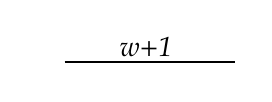
\begin{tikzpicture}
\foreach \x in {0}
\foreach \y in {0}
%{
%\draw (\x, \y)    rectangle ++(2,2);
%};
%\draw  (1,1.7) node{\protect{$#1$}};  %% north
%\draw (1.7,1) node{$\addone$}; %% east
\draw  (1,.3) node{\quad\underline{$\qquad \emph{w+1}\qquad$ }\quad};  %% south
\end{tikzpicture}
&
\domino{i+1}{k} 
& \begin{tikzpicture}
\foreach \x in {0}
\foreach \y in {0}
%{
%\draw (\x, \y)    rectangle ++(2,2);
%};
\draw  (1,2.7) node{\quad\underline{$\qquad ??\qquad$ }\quad}; 
%\draw (1.7,1) node{$\addone$}; %% east
\draw  (1,1.3) node{\quad\quad};  %% south
\end{tikzpicture}
&
\domino{k}{} \\
\!\!\!\!\!\!\!\!\!\!\!\!\!\!\!\!\!\!\!\!\!\!\!\!\!\!\!\!\!\!\!\!\!\!\!\! d_{n+1}   & d_{n+2} & & d_{n+3}
\end{array}
$
\end{flushleft}

\vfil\eject



\begin{flushleft}
$
\begin{array}{ccccc}
\domino{i}{1\quad 1+1} 
 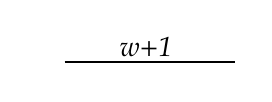
\begin{tikzpicture}
\foreach \x in {0}
\foreach \y in {0}
%{
%\draw (\x, \y)    rectangle ++(2,2);
%};
%\draw  (1,1.7) node{\protect{$#1$}};  %% north
%\draw (1.7,1) node{$\addone$}; %% east
\draw  (1,.3) node{\quad\underline{$\qquad \emph{w+1}\qquad$ }\quad};  %% south
\end{tikzpicture}
&
\domino{i+1}{k} 
& \begin{tikzpicture}
\foreach \x in {0}
\foreach \y in {0}
%{
%\draw (\x, \y)    rectangle ++(2,2);
%};
\draw  (1,2.7) node{\quad\underline{$\qquad ??\qquad$ }\quad}; 
%\draw (1.7,1) node{$\addone$}; %% east
\draw  (1,1.3) node{\quad\quad};  %% south
\end{tikzpicture}
&
\domino{k}{} \\
\!\!\!\!\!\!\!\!\!\!\!\!\!\!\!\!\!\!\!\!\!\!\!\!\!\!\!\!\!\!\!\!\!\!\!\! d_{n+1}   & d_{n+2} & & d_{n+3}
\end{array}
$
\end{flushleft}

\vfil\eject



\begin{flushleft}
$\begin{array}{ccccc}
\domino{}{i} 
 \begin{tikzpicture}
\foreach \x in {0}
\foreach \y in {0}
%{
%\draw (\x, \y)    rectangle ++(2,2);
%};
%\draw  (1,1.7) node{\protect{$#1$}};  %% north
%\draw (1.7,1) node{$\addone$}; %% east
\draw  (1,.3) node{\quad\underline{$\qquad w\qquad$ }\quad};  %% south
\end{tikzpicture}
&
\domino{i}{i + k } 
& \begin{tikzpicture}
\foreach \x in {0}
\foreach \y in {0}
%{
%\draw (\x, \y)    rectangle ++(2,2);
%};
\draw  (1,2.7) node{\quad\underline{$\quad \emph{w+1}\quad$ }\quad}; 
%\draw (1.7,1) node{$\addone$}; %% east
\draw  (1,1.3) node{\quad\quad};  %% south
\end{tikzpicture}
&
\domino{j=i+1}{k} \\
\!\!\!\!\!\!\!\!\!\!\!\!\!\!\!\!\!\!\!\!\!\!\!\!\!\!\!\!\!\!\!\!\!\!\!\! d_n   & d_{n+1} & & d_{n+2}
\end{array}
$
\end{flushleft}

\vfil\eject



\begin{flushleft}
$\begin{array}{l}
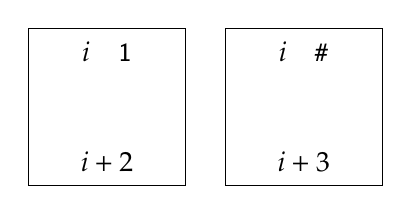
\begin{tikzpicture}
\foreach \x in {0,2.5}
\foreach \y in {0}
{
\draw (\x, \y)    rectangle ++(2,2);
};
\draw  (1,1.7) node{$i\quad {\one}$};  %% north
%\draw (1.7,1) node{$\addone$}; %% east
\draw  (1,.3) node{$i+2$};  %% south
 %\draw  (.3,1) node{$\addone$};   %% west
 %
\draw  (3.5,1.7) node{$i\quad  {\hash}$};  %% north
%\draw (4.2,1) node{$\addone$}; %% east
\draw  (3.5,.3) node{$i+3$};  %% south
% \draw  (2.8,1) node{$\one$};   %% west
 %
  \end{tikzpicture}
  \end{array}$
\end{flushleft}

\vfil\eject



\begin{flushleft}
$
\begin{array}{ccccc}
\domino{}{i} 
 \begin{tikzpicture}
\foreach \x in {0}
\foreach \y in {0}
%{
%\draw (\x, \y)    rectangle ++(2,2);
%};
%\draw  (1,1.7) node{\protect{$#1$}};  %% north
%\draw (1.7,1) node{$\addone$}; %% east
\draw  (1,.3) node{\quad\underline{$\qquad w\qquad$ }\quad};  %% south
\end{tikzpicture}
&
\domino{i \quad \hash}{i + 3 } 
& \begin{tikzpicture}
\foreach \x in {0}
\foreach \y in {0}
%{
%\draw (\x, \y)    rectangle ++(2,2);
%};
\draw  (1,2.7) node{\quad\underline{$\quad \emph{v}\quad$ }\quad}; 
%\draw (1.7,1) node{$\addone$}; %% east
\draw  (1,1.3) node{\quad\quad};  %% south
\end{tikzpicture}
&
\domino{j=i+3}{k} \\
\!\!\!\!\!\!\!\!\!\!\!\!\!\!\!\!\!\!\!\!\!\!\!\!\!\!\!\!\!\!\!\!\!\!\!\! d_n   & d_{n+1} & & d_{n+2}
\end{array}
$
\end{flushleft}

\vfil\eject



\begin{flushleft}
$\begin{array}{l}
 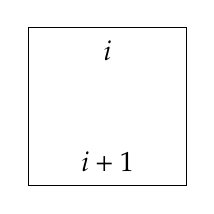
\begin{tikzpicture}
 \domino{i}{i+1}
  \end{tikzpicture}
\end{array}$
\end{flushleft}

\vfil\eject



\begin{flushleft}
$\begin{array}{l}
\begin{array}{ccccc}
\domino{}{i} 
 \begin{tikzpicture}
\foreach \x in {0}
\foreach \y in {0}
%{
%\draw (\x, \y)    rectangle ++(2,2);
%};
%\draw  (1,1.7) node{\protect{$#1$}};  %% north
%\draw (1.7,1) node{$\addone$}; %% east
\draw  (1,.3) node{\quad\underline{$\qquad w\qquad$ }\quad};  %% south
\end{tikzpicture}
&
\domino{i}{i + 1} 
& \begin{tikzpicture}
\foreach \x in {0}
\foreach \y in {0}
%{
%\draw (\x, \y)    rectangle ++(2,2);
%};
\draw  (1,2.7) node{\quad\underline{$\quad w\quad$ }\quad}; 
%\draw (1.7,1) node{$\addone$}; %% east
\draw  (1,1.3) node{\quad\quad};  %% south
\end{tikzpicture}
&
\domino{j=i+1}{k} \\
\!\!\!\!\!\!\!\!\!\!\!\!\!\!\!\!\!\!\!\!\!\!\!\!\!\!\!\!\!\!\!\!\!\!\!\! d_n   & d_{n+1} & & d_{n+2}
\end{array}
\end{array}$
\end{flushleft}
\vfil\eject





\begin{flushleft}
$\begin{array}{l}
\dominogreen{start}{start\ \numberone}
\quad
\dominothin{\one}{\one}
\quad
\dominothin{\hash}{\hash}
%\quad
%\dominothin{\one}{\inverse{\one}}
%\quad
%\dominothin{\hash}{\inverse{\hash}}
\end{array}$
\end{flushleft}

\vfil\eject



\begin{flushleft}
$\begin{array}{ll}
 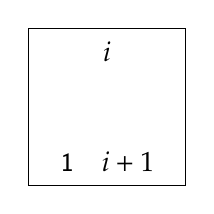
\begin{tikzpicture}
\foreach \x in {0}
\foreach \y in {0}
{
\draw (\x, \y)    rectangle ++(2,2);
};
\draw  (1,1.7) node{$i$};  %% north
%\draw (1.7,1) node{$\passthrough$}; %% east
\draw  (1,.3) node{\one\quad  $i+1$};  %% south
 %\draw  (.3,1) node{$\passthrough$};   %% west
 %
\end{tikzpicture}
&\qquad\qquad\qquad
 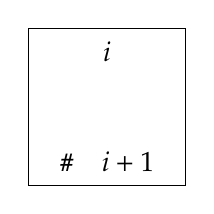
\begin{tikzpicture}
\foreach \x in {0}
\foreach \y in {0}
{
\draw (\x, \y)    rectangle ++(2,2);
};
\draw  (1,1.7) node{$i$};  %% north
%\draw (1.7,1) node{$\passthrough$}; %% east
\draw  (1,.3) node{\hash\quad $i+1$};  %% south
 %\draw  (.3,1) node{$\passthrough$};   %% west
 %
\end{tikzpicture}
\end{array}
$
\end{flushleft}

\vfil\eject



\begin{flushleft}
$\begin{array}{ll}
 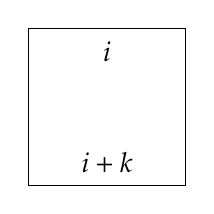
\begin{tikzpicture}
\foreach \x in {0}
\foreach \y in {0}
{
\draw (\x, \y)    rectangle ++(2,2);
};
\draw  (1,1.7) node{$i$};  %% north
%\draw (1.7,1) node{$\passthrough$}; %% east
\draw  (1,.3) node{$i+k$};  %% south
 %\draw  (.3,1) node{$\passthrough$};   %% west
 %
\end{tikzpicture}
&\qquad\qquad\qquad
 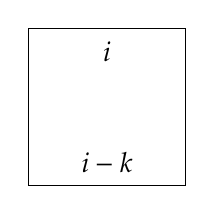
\begin{tikzpicture}
\foreach \x in {0}
\foreach \y in {0}
{
\draw (\x, \y)    rectangle ++(2,2);
};
\draw  (1,1.7) node{$i$};  %% north
%\draw (1.7,1) node{$\passthrough$}; %% east
\draw  (1,.3) node{$i-k$};  %% south
 %\draw  (.3,1) node{$\passthrough$};   %% west
 %
\end{tikzpicture}
\end{array}$
\end{flushleft}

\vfil\eject



\begin{flushleft}
$\begin{array}{l}
\domino{i}{i+1}%quad\mbox{halt}}{\mbox{halt}}
 \quad
 \begin{tikzpicture}
\foreach \x in {0,2.5}
\foreach \y in {0}
{
\draw (\x, \y)    rectangle ++(2,2);
};
\draw  (1,1.7) node{$i\quad {\one}$};  %% north
%\draw (1.7,1) node{$\addone$}; %% east
\draw  (1,.3) node{$i+2$};  %% south
 %\draw  (.3,1) node{$\addone$};   %% west
 %
\draw  (3.5,1.7) node{$i\quad  {\hash}$};  %% north
%\draw (4.2,1) node{$\addone$}; %% east
\draw  (3.5,.3) node{$i+3$};  %% south
% \draw  (2.8,1) node{$\one$};   %% west
 %
  \end{tikzpicture}
\end{array}$
\end{flushleft}

\vfil\eject



\begin{flushleft}
$\begin{array}{l}
\begin{tikzpicture}[remember picture,overlay]
\node [rotate=60,scale=1.7,text opacity=1.5]
%at (current page.center) {\emph{Pipe dream!}};
at (4.5,5.8) {\emph{Not this one!}};
\end{tikzpicture}
\end{array}$
\end{flushleft}

\vfil\eject



\begin{flushleft}
$\begin{array}{l}
\dominogreen{start}{start\quad\numberone}
\
\dominoblue{\numberone}{\one\quad 2}
\
\dominothin{\one}{\one}
\
\dominoblue{2}{\hash\quad 3}
\
\dominothin{\one}{\one}
\
\dominothin{\hash}{\hash}
\\
\dominoblue{3}{\hash\quad 4}
\
\dominothin{\one}{\inverse{\one}}
\
\dominothin{\hash}{\hash}
\
\dominothin{\hash}{\hash}
\
\dominoblue{4\quad $\inverse{\one}$}{3}
\
\dominothin{\hash}{\hash}
\
\dominothin{\hash}{\hash}
\
\\
\dominoblue{3}{\hash\quad 4}
\
\
\dominothin{\hash}{\inverse{\hash}}
\
\dominothin{\hash}{\hash}
\
\dominothin{\hash}{\hash}
\\
\dominoblue{4\quad $\inverse{\hash}$}{4}
\
\dominothin{\hash}{\inverse{\hash}}
\
\dominothin{\hash}{\hash}
\
\dominoblue{4\quad $\inverse{\hash}$}{4}
\
\dominothin{\hash}{\inverse{\hash}}
\
\dominoblue{4\quad $\inverse{\hash}$}{4}
\
\domino{4\quad halt}{halt}
\end{array}$
\end{flushleft}

\vfil\eject



\begin{flushleft}
$\begin{array}{l}
 \begin{tikzpicture}
\foreach \x in {0}
\foreach \y in {0}
{
\draw (\x, \y)    rectangle ++(2,2);
};
\draw  (1,1.7) node{$n$};  %% north
%\draw (1.7,1) node{$\passthrough$}; %% east
\draw  (1,.3) node{\one\  n+1};  %% south
 %\draw  (.3,1) node{$\passthrough$};   %% west
 %
\end{tikzpicture}
\end{array}$
\end{flushleft}

\vfil\eject



\begin{flushleft}
$\begin{array}{l}
\begin{tikzpicture}
\foreach \x in {0,2.5}
\foreach \y in {0}
{
\draw (\x, \y)    rectangle ++(2,2);
};
\draw  (1,1.7) node{$n\quad \inverse{\one}$};  %% north
%\draw (1.7,1) node{$\addone$}; %% east
\draw  (1,.3) node{next(n+2)};  %% south
 %\draw  (.3,1) node{$\addone$};   %% west
 %
\draw  (3.5,1.7) node{$n\quad \inverse{\hash}$};  %% north
%\draw (4.2,1) node{$\addone$}; %% east
\draw  (3.5,.3) node{next(n+3)};  %% south
% \draw  (2.8,1) node{$\one$};   %% west
 %
  \end{tikzpicture}
\end{array}$
\end{flushleft}

\vfil\eject



\begin{flushleft}
$\begin{array}{l}
\domino{}{x}
\  \dominothin{\hash}{\hash}
\  \dominothin{\one}{\one}
\ \domino{x}{\one \quad y}
\qquad ? \qquad
\domino{y}{\hash \quad z}
\end{array}$
\end{flushleft}

\vfil\eject


\begin{flushleft}
$\begin{array}{l}
\domino{}{x}
\  \dominothin{\hash}{\hash}
\  \dominothin{\one}{\one}
\ \domino{x}{\one \quad y}
\  \dominothin{\hash}{\hash}
\  \dominothin{\one}{\one}
\  \dominothin{\one}{\one}
\ \domino{y}{\hash \quad z}
\end{array}$
\end{flushleft}

\vfil\eject




\begin{flushleft}
$\begin{array}{l}
\domino{}{x}
\  \dominothin{\hash}{\hash}
\  \dominothin{\one}{\one}
\ \domino{x}{\one \quad y}
\qquad ? \qquad
\domino{y\quad \inverse{\hash}}{z}
\end{array}$
\end{flushleft}

\vfil\eject




\begin{flushleft}
$\begin{array}{l}
\domino{}{x}
\  \dominothin{\hash}{\inverse{\hash}}
\  \dominothin{\one}{\one}
\ \domino{x\quad \inverse{\hash}}{y}
\qquad ? \qquad
\ \domino{y}{\one\quad z}
\end{array}$
\end{flushleft}

\vfil\eject

\end{document}

\begin{flushleft}
$\begin{array}l}

\end{array}$
\end{flushleft}

\vfil\eject




\begin{flushleft}
$\begin{array}l}

\end{array}$
\end{flushleft}

\vfil\eject




\begin{flushleft}
$\begin{array}l}

\end{array}$
\end{flushleft}

\vfil\eject




\begin{flushleft}
$\begin{array}l}

\end{array}$
\end{flushleft}

\vfil\eject




\begin{flushleft}
$\begin{array}l}

\end{array}$
\end{flushleft}

\vfil\eject




\begin{flushleft}
$\begin{array}l}

\end{array}$
\end{flushleft}

\vfil\eject




\begin{flushleft}
$\begin{array}l}

\end{array}$
\end{flushleft}

\vfil\eject




\begin{flushleft}
$\begin{array}l}

\end{array}$
\end{flushleft}

\vfil\eject




\begin{flushleft}
$\begin{array}l}

\end{array}$
\end{flushleft}

\vfil\eject




\begin{flushleft}
$\begin{array}l}

\end{array}$
\end{flushleft}

\vfil\eject




\begin{flushleft}
$\begin{array}l}

\end{array}$
\end{flushleft}

\vfil\eject




\begin{flushleft}
$\begin{array}l}

\end{array}$
\end{flushleft}

\vfil\eject




\begin{flushleft}
$\begin{array}l}

\end{array}$
\end{flushleft}

\vfil\eject




\begin{flushleft}
$\begin{array}l}

\end{array}$
\end{flushleft}

\vfil\eject






































\end{document}